\documentclass[conference]{IEEEtran}

\usepackage{times}
\usepackage{epsfig}
\usepackage{amsmath}
\usepackage{amssymb}
\usepackage{graphicx}
\usepackage[font=footnotesize]{caption}
\usepackage{subcaption} 
\usepackage{amsmath,amssymb,amsthm}
\usepackage{algorithm}
\usepackage{color}
\definecolor{light-gray}{gray}{0.4}
\usepackage[noend]{algpseudocode} 
%\usepackage[noadjust]{cite}
\usepackage[sort&compress,numbers]{natbib} % required by RSS

\pdfminorversion=5
\pdfobjcompresslevel=3 
\pdfcompresslevel=9 

% list of commenters
\newcommand{\ssnote}[1]{{\xxnote{SS}{red}{#1}}}
% implement conditional notes (turn on/off with \hidenotes above)
\newcommand{\xxnote}[3]{}
\ifx\hidenotes\undefined
  \renewcommand{\xxnote}[3]{\color{#2}{#1: #3}}
\fi

% Labels in IEEE format
% Equation
\newcommand{\eref}[1]{(\ref{#1})}
% Section
\newcommand{\sref}[1]{Section~\ref{#1}}
% Figure
\newcommand{\figref}[1]{Fig.\ref{#1}}
% Table
\newcommand{\tabref}[1]{Table~\ref{#1}}
% Algorithm
\newcommand{\algoref}[1]{Alg.\ref{#1}}


\newcommand{\naive}{baseline\xspace}
\newcommand{\ie}{\textit{i.e.}\xspace}
\newcommand{\eg}{\textit{e.g.}\xspace}
\newcommand{\etal}{\textit{et al.}\xspace}
\newcommand{\Tango}{\textit{Tango}\xspace}
\newcommand{\TSDF}{TSDF\xspace}

\newif\iffinalcopy
\finalcopyfalse % or


\usepackage{xspace} 
\newcommand{\chisel}{\textsc{Chisel}\xspace}

\usepackage{booktabs} % Pretty tabular
\usepackage{multirow} % Cells that span multiple rows


% Include other packages here, before hyperref.

% If you comment hyperref and then uncomment it, you should delete
% egpaper.aux before re-running latex.  (Or just hit 'q' on the first latex
% run, let it finish, and you should be clear).
\usepackage[pagebackref=true,breaklinks=true,letterpaper=true,colorlinks,bookmarks=false]{hyperref}

\begin{document}

%%%%%%%%% TITLE
\title{\Large \chisel : Real Time Large Scale 3D Reconstruction Onboard a Mobile
Device
\\
using Spatially-Hashed Signed Distance Fields}

\newcommand{\fix}{\marginpar{FIX}}
\newcommand{\new}{\marginpar{NEW}}

\algnewcommand{\LineComment}[1]{\State \(\triangleright\)
\textcolor{light-gray}{\textit{#1}}}

%\nipsfinalcopy % Uncomment for camera-ready version

\iffinalcopy
	\author
	{
		Matthew Klingensmith \\
		Carnegie Mellon Robotics Institute\\
		\texttt{mklingen@andrew.cmu.edu}
		\and
		Ivan Dryanovski \\
		The Graduate Center,\\
		City University of New York\\
		\texttt{idryanovski@gc.cuny.edu}
		\and
		Siddhartha S. Srinivasa \\
		Carnegie Mellon Robotics Institute\\
		\texttt{siddh@cs.cmu.edu}
		\and
		Jizhong Xiao \\
		The City College of New York \\
		\texttt{jxiao@ccny.cuny.edu}
	} 
\else
	\author{\Large{Author names omitted for review. Paper Number 32} \\
	\small{\textit{Note to reviewers, a high resolution video is
available at:} \url{http://vimeo.com/117544631}}}
\fi

\maketitle

\thispagestyle{empty}

\begin{abstract}
We describe a system for real-time house-scale (300 square meter or more)
dense 3D reconstruction  onboard a  Google \Tango
\cite{Tango} mobile device by using a dynamic spatially-hashed truncated
signed distance field\cite{NiessnerHashing} for mapping, and visual-inertial
odometry for localization. By aggressively culling parts of
the scene that do not contain surfaces, we avoid needless computation and wasted
memory. Even under very noisy conditions, we produce high-quality
reconstructions through the use of space carving. We are able to reconstruct and
render very large scenes at a resolution of 2-3 cm in real
time on a mobile device without the use of GPU computing. The user is able to
view and interact with the reconstruction in real-time through an intuitive
interface. We provide both qualitative and quantitative results on publicly
available RGB-D datasets \cite{FREIBURG}, and on datasets collected in
real-time from two devices, as well as a motivating example involving an aerial
robot.

% reality and indoor building scanning applications
% Google's \textit{Project Tango}\cite{Tango} has made integrated depth sensing
% and onboard visual-inertial odometry \cite{VINS} available to mobile devices such
% as phones and tablets. In this work, we explore the problem of dense,
% large-scale 3D realtime reconstruction on a mobile device with integrated
% depth sensing. Solving this problem is a necessary pre-requisite for many indoor navigation, augmented
% reality and indoor building scanning applications.  Existing 3D reconstruction approaches on mobile
% devices either only build a sparse reconstruction \cite{KleinSparse}, offload
% their computation to other devices \cite{DTAM}, or require seconds-long
% post-processing per frame \cite{TanskanenMetric}.  state-of-the-art approaches
% in large-scale dense reconstruction \cite{Newcombe, Whelan2013} require large
% amounts of memory and high-performance GPU computing, which is often
% unavailable on mobile devices. Our approach accomplishes large-scale
% reconstruction on a mobile device by exploiting visual inertial odometry and by
% using chunked, dynamic spatial hash maps \cite{SpatialHashing} of truncated
% signed distance volumes \cite{Curless1996},  we are able to reconstruct and
% render very large (300 square meter) scenes at a resolution of 2-3cm in real
% time on a mobile device using only the CPU, with a memory footprint that is
% approximately 84 percent smaller than \textit{Kinect Fusion} \cite{Newcombe}. 
% We provide both qualitative and  quantitative results on publicly available
% RGB-D datasets \cite{FREIBURG}, and on datasets collected in real-time from two
% devices.
\end{abstract}

\section{Introduction}
Recently, mobile phone manufacturers have started adding
high-quality depth and  inertial sensors to mobile phones and tablets. In
particular, the devices we use in this work, Google's \Tango \cite{Tango}
phone and tablet have very small active infrared projection depth sensors
combined with high-performance IMUs and wide field of view cameras
(\sref{section:hardware}). Other devices, such as the Occiptal Inc.
\textit{Structure Sensor} \cite{StructureSensor} have similar capabilities.
These devices offer an onboard, fully integrated sensing platform for 3D mapping
and localization, with applications ranging from mobile robots to handheld,
wireless augmented reality. 

Real-time 3D reconstruction is a well-known problem in computer vision and
robotics \cite{Hartley2004}. The task is to extract the true 3D geometry of a
real scene from a sequence of noisy sensor readings online. Solutions to this
problem are useful for navigation, mapping, object scanning, and more. The
problem can be broken down into two components: localization (\ie estimating
the sensor's pose and trajectory), and mapping (\ie reconstructing the scene
geometry and texture).

Consider house-scale (300 square meter) real-time 3D mapping and localization on
a \Tango device.  A user (or robot) moves around a building, scanning
the scene. At house-scale, we are only concerned with features with a resolution
of about 2-3 cm (walls, floors, furniture, applicances, etc.). To facilitate
scanning, real-time feedback is given to the user on the device's screen.  The
user can export the resulting 3D scan without losing any data.
\figref{fig:first_figure} shows an example of this use case (\sref{section:mapping})
in progress. As an application of house-scale mapping, we consider a small
flying robot equipped with a \Tango sensor onboard (\figref{fig:robot}). The
robot must navigate indoor spaces by mapping them online (\sref{section:robot}).
Having all of the sensing and processing onboard the robot reduces the need for
streaming sensor data to offboard devices.

\begin{figure}[t!]
  \centering
    	 \begin{subfigure}{\linewidth} \centering
		 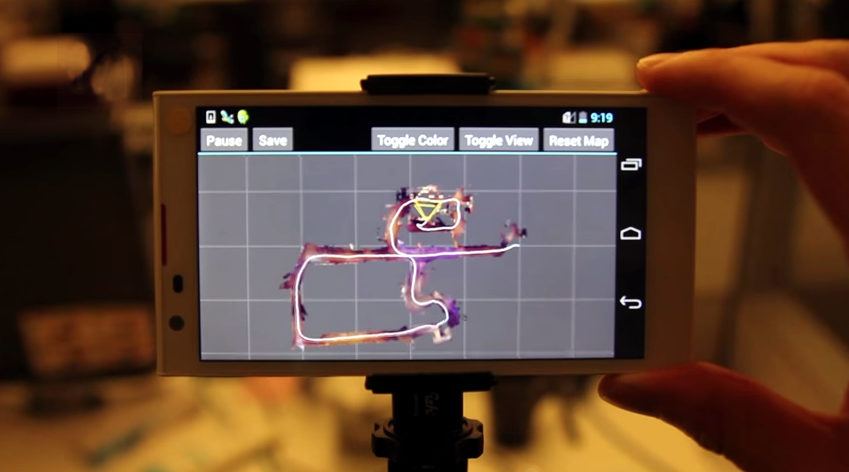
\includegraphics[width=0.75\textwidth]{img/mapdevice}
		 \caption{\chisel creating a map
      of an entire office building floor on a mobile device in real-time.}
		 \label{fig:map_device}
	 \end{subfigure}
      	 \begin{subfigure}{\linewidth} \centering
		 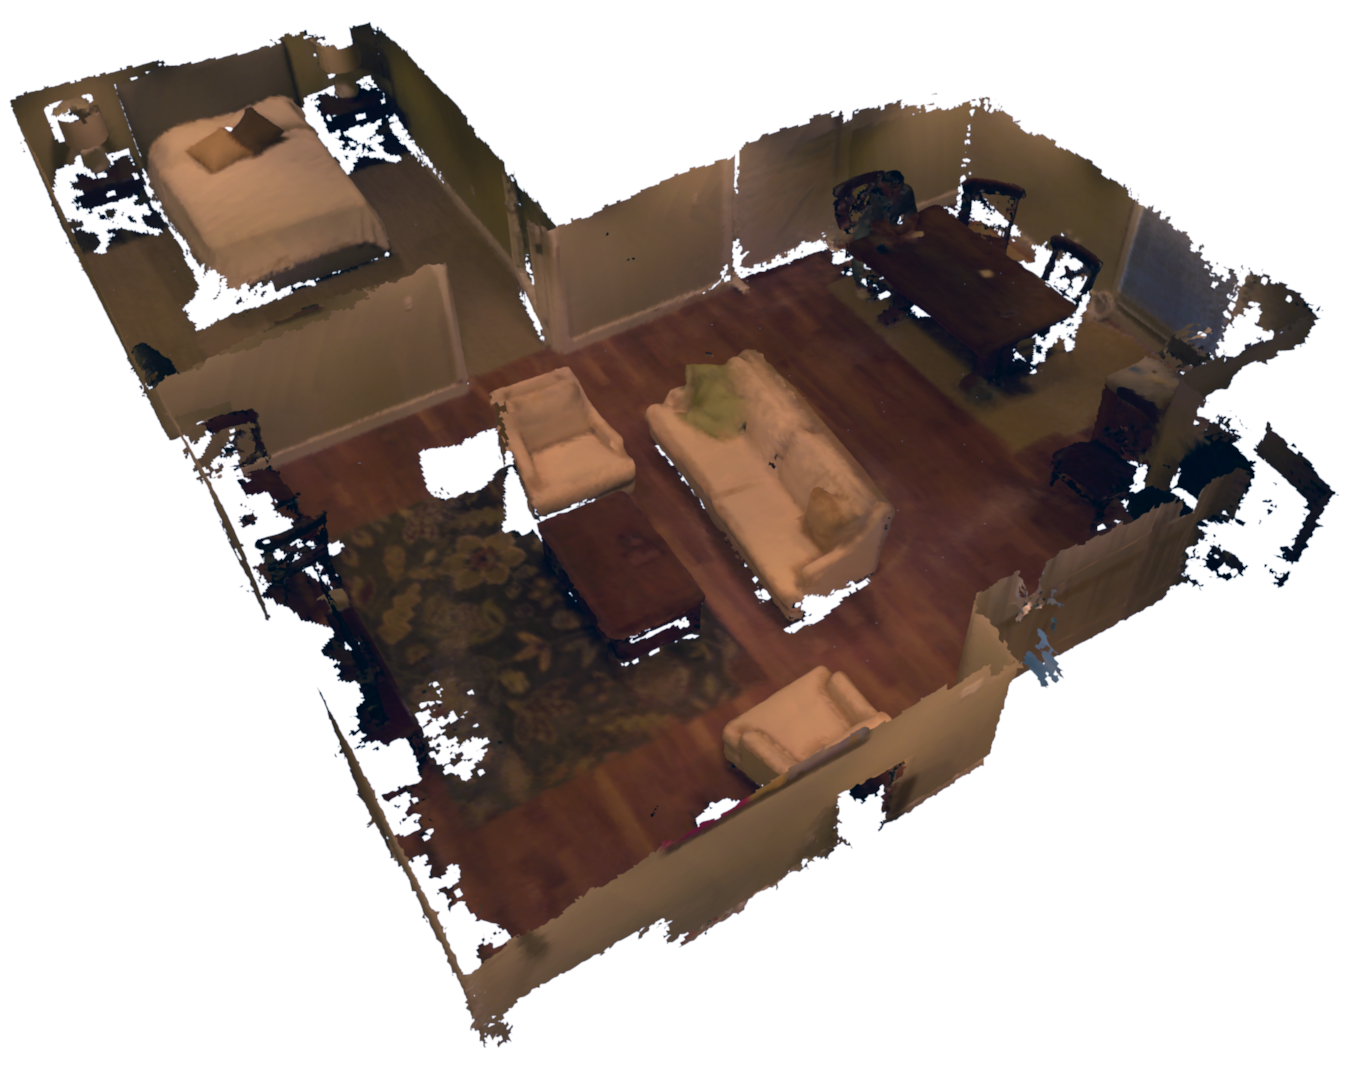
\includegraphics[width=0.75\textwidth]{img/apartment_scene_color.png}
		 \caption{Reconstructed apartment scene at a voxel resolution of 2cm.}
		 \label{fig:apartment_color}
	 \end{subfigure}
      \caption{\chisel running on Google's \Tango~\cite{Tango} device.}
  \label{fig:first_figure}
\end{figure} 

These use cases require that the 3D reconstruction algorithm must run entirely
onboard; fast enough to allow real-time interaction. Importantly, the entire
dense 3D reconstruction must fit inside the device's limited (2-4GB) memory
(\sref{section:hardware}). Because some mobile devices  lack sufficiently
powerful discrete graphics processing units (GPU), we choose not to rely on general
purpose GPU computing to make the problem tractable in either creating or
rendering the 3D reconstruction.

3D mapping algorithms involving occupancy grids \cite{Elfes1989}, keypoint
mapping \cite{KleinSparse} or point clouds \cite{RusinkiewiczPoints,
TanskanenMetric, WeiseScanning} already exist for mobile phones at small scale
-- but at the scales we are interested in, their reconstruction quality is
limited. Occupancy grids suffer from aliasing and are memory-dense, while
point-based methods cannot reproduce surface or volumetric features of the scene
without intensive post-processing.

Many state-of-the-art real-time 3D reconstruction algorithms \cite{Newcombe,
Whelan2013,WhelanLoopClose,Bylow2013,NiessnerHashing} compute a truncated
signed distance field (\TSDF) \cite{Curless1996} of the scene. The \TSDF stores a
discretized estimate of the distance to the nearest surface in the scene. While
allowing for very high-quality reconstructions, the \TSDF is very
memory-intensive. The size of the \TSDF needed to reconstruct an entire house
may be on the order of several gigabytes  (\sref{section:memory}), and
rendering the resulting reconstruction in real-time would certainly overwhelm
the graphics capabilities of a mobile phone. Previous works \cite{Whelan2013,
WhelanLoopClose} have extended the \TSDF to larger scenes by storing a
\textit{moving} voxelization and throwing away data incrementally -- but we are
interested in preserving the volumetric data for later use.

Experimentally, we found that most ( $\sim 93\%$) of the space in a typical
scene is in fact empty (\tabref{table:volumecount}). Iterating over empty space
for the puposes of reconstruction and rendering wastes computation time; and storing it
wastes memory. Noting this fact, we make use of a data structure introduced by
Niessner \etal \cite{NiessnerHashing}, the Dynamic spatially-hashed
\cite{SpatialHashing} \TSDF (\sref{section:spatialhash}), which stores the
distance field data as a two-level structure in which static 3D voxel
\textit{chunks} are dynamically allocated according to observations
of the scene. Because the data structure has $\mathcal{O}(1)$ access
performance, we are able to quickly identify which parts of the scene should be
rendered, updated, or deleted. This allows us to minimize the amount of time we
spend on each depth scan and keep the reconstruction running in real-time on the device.

For localization, we use a mix of  visual-inertial odometry \cite{VINS, VINS2}
and sparse keypoint-based mapping \cite{FastSlam} as a black box
(\sref{section:pose}). These approaches use only the 2D wide-angle camera and
the IMU, and take in no information from the depth sensor. As a consequence,
our mapping system  is \textit{open-loop} in the sense that it does not attempt
to explicitly estimate the pose of the sensor from the 3D reconstruction. In spite
of this limitation, we found that using  open-loop visual odometry was
sufficient to create high-quality, house-scale reconstructions
(\figref{fig:night3}). Additionally  the user can post-process the model using
global optimization of the trajectory through bundle adjustment, which our
system can also do on-device

 We provide qualitative and  quantitative results on publicly available RGB-D
 datasets \cite{FREIBURG}, and on datasets collected in real-time from two
 devices (\sref{section:experiments}). We compare different approaches for
 creating (\sref{section:scan_compare}) and storing (\sref{section:memory}) the
 \TSDF in terms of memory efficiency, speed, and reconstruction quality. Our
 system (called \chisel), is able to produce high-quality, large scale 3D
 reconstructions of outdoor and indoor scenes in real-time onboard a mobile device.

\section{Related Work}
Mapping paradigms generally fall into one of two categories: landmark-based (or
\emph{sparse}) mapping, and high-resolution \emph{dense} mapping
\cite{FastSlam}.  While sparse mapping generates a metrically consistent map of
landmarks based on key features in the environment, dense mapping globally
registers all sensor data into a high-resolution data structure. In this work,
we are concerned primarily with dense mapping, which is essential for high
quality 3D reconstruction.

Because mobile phones typically do not have depth sensors, previous works
\cite{TanskanenMetric, DTAM, LSDSlam} on dense reconstruction for mobile phones
have gone to great lengths to extract depth from a series of registered monocular camera
images. Since our work focuses on mobile devices with integrated depth sensors,
such as the Google \Tango devices \cite{Tango}, we do not need to perform
costly monocular stereo as a pre-requisite to dense reconstruction. This allows
us to save our memory and CPU budget for the 3D reconstruction itself.

One of the simplest means of dense 3D mapping is storing multiple registered
point clouds. These point-based methods \cite{RusinkiewiczPoints,
TanskanenMetric, WeiseScanning, LSDSlam} naturally convert depth data into
projected 3D points. While simple, point clouds fail to capture local scene
structure, are noisy, and fail to capture \emph{negative} (non-surface)
information about the scene. This information is crucial to scene reconstruction
under high levels of noise \cite{Klingensmith2014}.

Elfes \cite{Elfes1989} introduced Occupancy Grid Mapping, which divides the
world into a voxel grid containing occupancy probabilities. Occupancy grids
preserve local structure, and gracefully handle redundant and missing data.  
While more robust than point clouds, occupancy grids suffer from aliasing, and
lack information about surface normals and the interior/exterior of obstacles. 
Occupancy grid mapping has already been shown to perform in real-time on \Tango
\cite{Tango} devices using an Octree representation \cite{Wurm2010}.

% Attempts to extend occupancy grid maps to 3D have sometimes relied on octrees.
% Rather than storing a fixed-resolution grid, octrees store occupancy data in a
% spatially organized tree. In typical scenes, octrees reduce the required memory
% over occupancy grids by orders of magnitude. Octomap \cite{Wurm2010} is a
% popular example of the octree paradigm. However, octrees containing only
% occupancy probability suffer from many of the same problems as occupancy grids:
% they lack information about the interior and exterior of objects, and suffer
% from aliasing. Further, octrees suffer from logarithmic reading, writing, and
% iteration times, and have very poor memory locality characteristics.

Curless and Levoy \cite{Curless1996} created an alternative to occupancy
grids called the Truncated Signed Distance Field (\TSDF), which stores a
voxelization of the signed distance field of the scene. The \TSDF is negative
inside obstacles, and positive outside obstacles. The surface is given
implicitly as the zero isocontour of the \TSDF. While using more memory
than occupancy grids, the \TSDF creates much higher quality surface
reconstructions by preserving local structure.

In robotics, distance fields are used in motion planning
\cite{RatliffChomp}, mapping \cite{VandapelKA05}, and scene understanding.
Distance fields provide useful information to robots: the distance to the
nearest obstacle, and the gradient direction to take them away from obstacles. 
A recent work by Wagner \etal \cite{WagnerICRA13} explores the direct use of a
\TSDF for robot arm motion planning; making use of the gradient information
implicitly stored in the \TSDF to locally optimize robot trajectories. We are
interested in similarly planning trajectories for autonomous flying robots by
directly using \TSDF data (\sref{section:robot}). Real-time onboard 3D mapping,
navigation and odometry has already been achieved on flying robots
\cite{FlyingNavigation, OSMAV}using occupancy grids. Our system is
complimentary to this work.

\emph{Kinect Fusion} \cite{Newcombe} uses a \TSDF to simultanesously extract the
pose of a moving depth camera and scene geometry in real-time. Making
heavy use of the GPU for scan fusion and rendering, \textit{Fusion} is capable
of creating extremely high-quality, high-resolution surface reconstructions within
a small area. However, like occupancy grid mapping, the algorithm relies on a
single fixed-size 3D voxel grid, and thus is not suitable for reconstructing
very large scenes due to memory constraints. This limitation has generated
interest in extending  \TSDF fusion to larger scenes. 
Moving window approaches, such as \emph{Kintinuous} \cite{Whelan2013} extend
Kinect Fusion to larger scenes by storing  a moving voxel grid in the GPU. As
the camera moves outside of the grid, areas which are no longer visible are
turned into a surface representation. Hence, distance field data is prematurely 
thrown away to save memory. As we want to save distance field data so it can be
used later for post-processing, motion planning, and other applications, a
moving window approach is not suitable.

Recent works have focused on extending \TSDF fusion to larger scenes by
compressing the distance field to avoid storing and iterating
over empty space. Many have used \textit{hierarichal} data structures such as
octrees or KD-trees to store the \TSDF \cite{Zeng2012, Chen2012}. However, these
structures suffer from high complexity and complications with parallelism. 

An approach by Niessner \etal \cite{NiessnerHashing} uses a two-layer
hierarichal data structure that uses spatial hashing \cite{SpatialHashing} to
store the \TSDF data. This approach avoids the needless complexity of other
hierarchical data structures, boasting $\mathcal{O}(1)$ queries, and avoids
storing or updating empty space far away from surfaces.

Our system adapts the spatially-hashed data structure of
Niessner \etal \cite{NiessnerHashing} to \Tango devices. By carefully
considering what parts of the space should be turned into distance fields at
each timestep, we avoid needless computation (\tabref{table:meshingtimes}) and
memory allocation (\figref{fig:memory_data}) in areas far away from the sensor.
Unlike \cite{NiessnerHashing}, we do not make use of any general purpose GPU
computing. All \TSDF fusion is performed on the mobile processor, and the
volumetric data structure is stored on the CPU. Instead of rendering the scene
via raycasting, we generate polygonal meshes incrementally for only the parts
of the scene that need to be rendered. Since the depth sensor found on the
\Tango device is significantly more noisy than other commercial depth
sensors, we reintroduce space carving \cite{Elfes1989} from occupancy grid
mapping (\sref{section:carving}) and dynamic trunction
(\sref{section:dynamic_trunc}) into the \TSDF fusion algorithm to improve
reconstruction quality under conditions of high noise. The space carving and
truncation algorithms are informed by a parametric noise model trained for the
sensor using the method of Nguyen \etal \cite{Nguyen2012}.

\section{System Implementation} 
\subsection{Preliminaries}
\label{section:prelim}
Consider the geometry of the ideal pinhole depth sensor. Rays emanate from the
sensor origin to the scene.  \figref{fig:raycast_diagram} is a diagram of a ray hitting a
 surface from the camera, and a voxel that the ray passes through.  Call  the
 origin of the ray $o$, and the endpoint of the ray $\mathbf{x}$.
The length of the ray is given by $z = \|\mathbf{o}
- \mathbf{x}\|$. The direction of the ray is given by $\mathbf{\hat{r}} =
\frac{\mathbf{o} - \mathbf{x}}{z}$. The endpoint of each ray represents a point
on the surface.  We can also parameterize the ray by its direction and
endpoint, using an interpolating parameter $u$:

 \begin{equation}
 	\mathbf{v}(u) = \mathbf{x} - u\mathbf{\hat{r}}
 \end{equation}

At each timestep $t$ we have a set of rays $Z_t$. In practice, the rays are
corrupted by noise. Call $d$ the true distance from the origin of the sensor to
the surface along the ray. Then $z$ is actually a random variable drawn from a
distribution dependant on $d$ called the \textit{hit probability}
(\figref{fig:integration_diagram}). Assuming the hit probability is Gaussian, we
have:

\begin{equation}
\label{eqn:hitprobability}
z \sim \mathcal{N}(d, \sigma_d)
\end{equation}

\noindent where $\sigma_d$ is the standard deviation of the depth noise for a
true depth $d$. We train this model using a method from \textit{Nguyen} \etal
\cite{Nguyen2012}.

Another complication is that since depth sensors are not ideal, an actual depth
reading corresponds to many possible rays through the scene. Therefore, each
depth reading represents a \textit{cone}, rather than a ray. The ray passing
through the center of the cone closely approximates it near the sensor, but the
approximation gets worse further away.

% Rays are in practice stored in a 2D depth image at each timestep. We can
% calibrate the depth sensor as a pinhole camera with camera intrinsics $\{f_x,
% f_y, c_x, c_y\}$. Using the intrinsics, we can project onto the camera plane
% using the pinhole model. The function $\mathbf{Project} :
% \mathbf{R}^3\to\mathbf{R}^2$ accomplishes this. We can also bilinearly
% interpolate points in the depth image. The function $\mathbf{InterpolateDepth}
% : \mathbf{R}^2 \to \mathbf{R}^+$ does this.

\subsection{The Truncated Signed Distance Field}
\label{section:TSDF}
We model the world~\cite{Curless1996} as a volumetric signed distance field $\Phi: \mathbf{R}^3
\to \mathbf{R}$. For any point in the world $x$, $\Phi(x)$
is the distance to the nearest surface, \emph{signed} positive if the point is
outside of obstacles and negative otherwise. Thus, the zero isocontour $(\Phi =
0)$ encodes the surfaces of the scene.

Since we are mainly interested in reconstructing surfaces,
we use the Truncated Signed Distance Field (\TSDF) \cite{Curless1996}:
\begin{equation}
	\Phi_{\tau}(\mathbf{x}) =
	\begin{cases}
		\Phi(\mathbf{x}) &  \text{if} |\Phi(\mathbf{x})| < \tau \\
		\text{undefined} & \text{otherwise}
	\end{cases}
\end{equation}
where $\tau \in \mathbf{R}$ is the \emph{truncation distance}.  Curless and
Levoy \cite{Curless1996} note that very near the endpoints of depth rays, the
\TSDF is closely approximated by the distance along the ray to the nearest observed
point.   
 
% Furthermore, computing the first-order Taylor series approximation of $\Phi_{\tau}$
% about a point on the surface $\mathbf{x}_s$, we get:
% \begin{align}
% \label{eqn:atsdf}
% \Phi_{\tau}(\mathbf{x}) &\approx \Phi_{\tau}(\mathbf{x}_s) + \nabla \Phi(\mathbf{x}_s)^{T} (\mathbf{x} - \mathbf{x}_s) \nonumber \\
%  &= \nabla \Phi(\mathbf{x}_s)^{T} (\mathbf{x} - \mathbf{x}_s) = \mathbf{\hat{n}}(\mathbf{x}_s)^{T}(\mathbf{x} - \mathbf{x}_s)
% \end{align}
% where we denote $\nabla \Phi(\mathbf{x}_s) = \mathbf{\hat{n}}(\mathbf{x}_s)$, the unit surface normal at $\mathbf{x}_s$, 
% encoding the observation that $\Phi$ changes fastest along the surface normal, and $||\nabla \Phi|| = 1$.
% 
% Now consider a ray from an ideal (noise-free) pinhole depth sensor with origin at $\mathbf{o}$ that 
% hits the surface at $\mathbf{x}_s$. Not only does this ray provide the measurement $\mathbf{x}_s$,
% it also carves out empty space from $\mathbf{o}$ to $\mathbf{x}_s$.  First, we parametrize the ray as 
% \begin{equation}
% \mathbf{x}(u) = \mathbf{x}_s - u\mathbf{\hat{r}}
% \end{equation}
% where $u \in \mathbf{R}$ and $\mathbf{\hat{r}}$ is the unit vector from $\mathbf{o}$ to $\mathbf{x}_s$.
% 
% Then, we use \eref{eqn:atsdf} to approximate $\Phi$ along the ray as (\figref{fig:raycast_diagram})
% \begin{equation}
% \Phi_{\tau}(\mathbf{x}(u)) \approx \mathbf{\hat{n}}(\mathbf{x}_s)^{T}(\mathbf{x}_s - u\mathbf{\hat{r}} - \mathbf{x}_s)
% = -u\mathbf{\hat{n}}(\mathbf{x}_s)^{T}\mathbf{\hat{r}}
% \end{equation}
% 
% Some works \cite{Bylow2013} approximate
% $\mathbf{\hat{n}}$ by locally fitting a plane around $\mathbf{x}_s$, but this comes at the cost of 
% computation. \ssnote{My rewrite stops here. Confused.}
% 
% Consider the geometry of the ideal pinhole depth sensor. Rays emanate from the
% sensor origin to the scene. At each timstep $t$ we have a set of rays
% $Z_t$. Call the origin of the ray $o$, and the endpoint of the ray $\mathbf{x}$.
% The length of the ray is given by $z = \|\mathbf{o}
% - \mathbf{x}\|$. The direction of the ray is given by $\mathbf{\hat{r}} =
% \frac{\mathbf{o} - \mathbf{x}}{z}$. The endpoint of each ray represents a point
% on the surface. So if  the sensor is perfect, we know that the signed distance
% function $\Phi(\mathbf{x}) = 0$ at that point. In practice, the ray is
% corrupted by noise. Call $d$ the true distance from the origin of the sensor to
% the surface along the ray. Then $z$ is actually a random variable drawn from a
% distribution dependant on $d$ called the \textit{hit probability}
% (\figref{fig:integration_diagram}).
% 
% The ray also implies that all the points in space along the ray from the sensor
% origin up to the endpoint must be outside of any surface (or else the ray would
% have been occluded by a a surface). Because real objects have non-zero
% thickness, some part of the space along the ray beyond the endpoint will be
% inside an object.
% 
% Further, very near the surface of the object, the signed distance field can
% be approximated by the distance along the ray to the endpoint of  the ray
% (\figref{fig:raycast_diagram}). Near $\mathbf{x}$, the signed distance field
% is approximately the distance to $\mathbf{x}$. So, whenever $|u|$ is very
% small:
% 
% \begin{equation} 
% \label{eq:pointwise_tsdf} 
% 	\Phi(\mathbf{x} - u\mathbf{\hat{r}}) \approx u 
% \end{equation}
% 
% The approximation is better whenever the ray is approximately
% perpendicular to the surface, and worst whenever the ray is parallel to the
% surface. Because of this, some works \cite{Bylow2013} instead approximate
% $\Phi$ by locally fitting a plane around $\mathbf{x}$ using the neighboring
% points and using the distance to that plane as a local approximation, \ie:
% 
% \begin{equation} 
% \label{eq:planar_tsdf} 
% 	\Phi(\mathbf{x} - u\mathbf{\hat{r}}) \approx -u~\mathbf{\hat{r}} \cdot
% 	\mathbf{\hat{n}_x}
% \end{equation}
% 
% \noindent where $\mathbf{\hat{n}_x}$ is the local surface normal around
% $\mathbf{x}$. In general, the planar approximation (\eref{eq:planar_tsdf})
% is much better than the pointwise approximation (\eref{eq:pointwise_tsdf}),
% especially when surfaces are nearly parallel to the sensor -- but computing surface normals is not
% always computationally feasible. In our work, we have chosen to use
% the simpler pointwise approximation.

\begin{figure*}
   \begin{subfigure}{1.0\columnwidth}
     \centering
         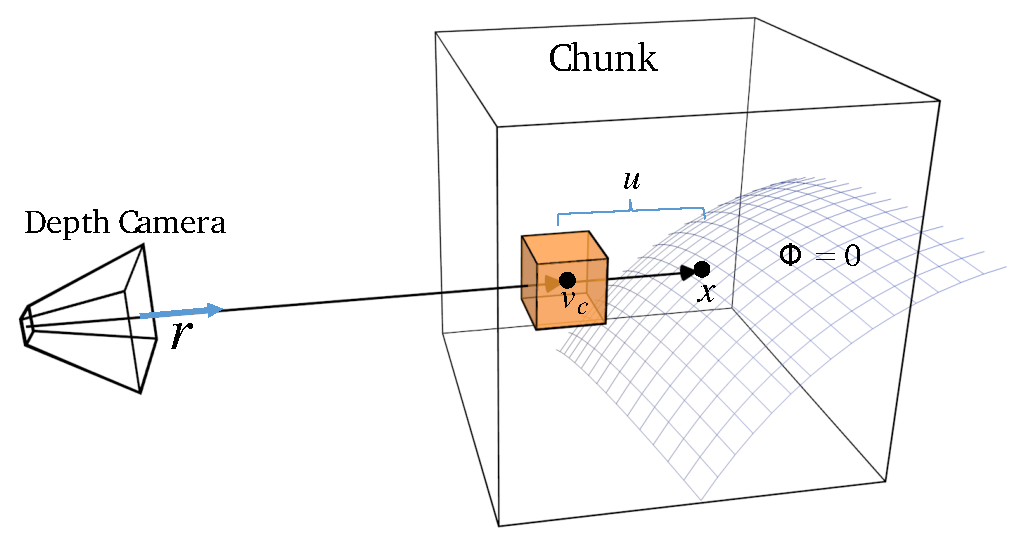
\includegraphics[width=1.0\textwidth]{img/Raycast}
      \caption{Raycasting through a voxel.}
  \label{fig:raycast_diagram}
   \end{subfigure}
      \begin{subfigure}{1.0\columnwidth}
     \centering
         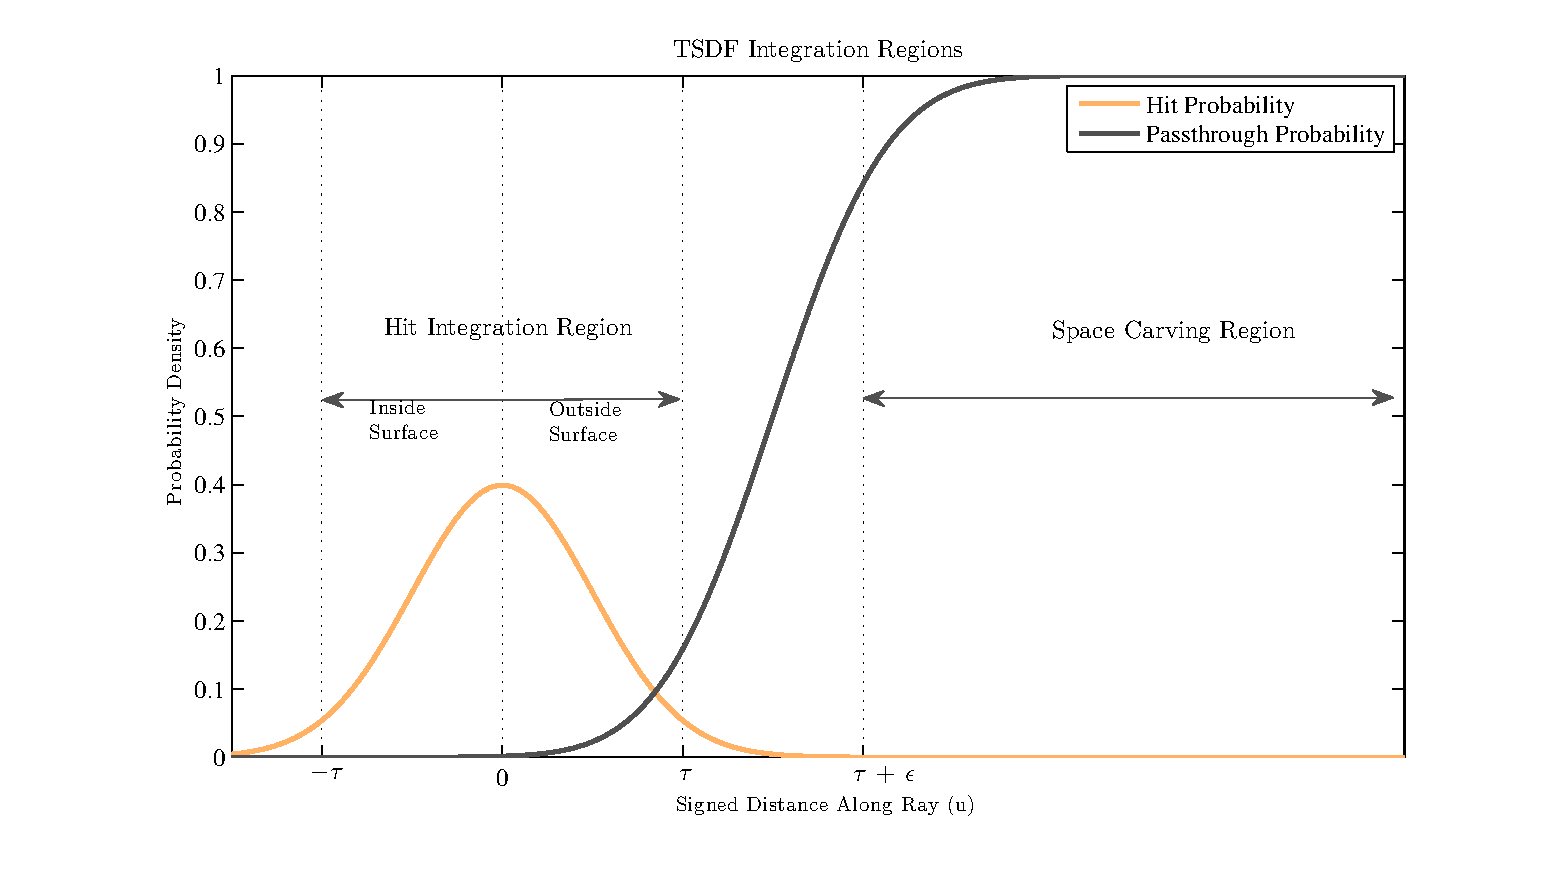
\includegraphics[ width=1.0\textwidth]{img/tsdf_integration.pdf}
         \caption{Noise model and the space carving region.}
  \label{fig:integration_diagram}
   \end{subfigure}
   \caption{Computing the Truncated Signed Distance Field (\TSDF).}
\end{figure*} 
% 
% This observation leads to the Truncated Signed Distance Field (TSDF)
% \cite{Curless1996}. The TSDF is defined as:
% 
% \begin{equation}
% 	\Phi_{\tau}(\mathbf{x}) = 
% 	\begin{cases}
% 		\Phi(\mathbf{x}) &  \text{if} |\Phi(\mathbf{x})| < \tau \\
% 		\text{undefined} & \text{otherwise}
% 	\end{cases}
% \end{equation} 
% 
% \noindent where $\tau \in \mathbf{R}$ is the ``truncation distance'' in which
% the TSDF is defined. Following \cite{Curless1996}, to update the TSDF with a
% particular sensor measurement, we update each voxel along the ray from $u =
% -\tau$ to $\tau$, and take the weighted running average of distance field estimates over time. To do
% this, we can introduce a global weighting function $W : \mathbf{R}^3 \to
% \mathbf{R^{+}}$ that represents the confidence in the estimate of the TSDF at
% every point in space.

\begin{algorithm}[t!]
	\caption{Truncated Signed Distance Field}
	\label{alg:TSDF}
	\begin{algorithmic}[1]
		\For {$t \in [1 \ldots T]$} \Comment{\textit{For each timestep}}
			\For {$\{\mathbf{o}_t, \mathbf{x}_t\} \in Z_t$} \Comment{\textit{For each ray in scan}}
				\State {$z \gets   \|\mathbf{o}_t - \mathbf{x}_t\|$}
				\State {$\mathbf{r} \gets \frac{\mathbf{x}_t - \mathbf{o}_t}{z}$}
				\State{$\tau \gets \mathcal{T} (z)$} \Comment{\textit{Dynamic truncation distance}}
				\label{alg:line:dynamic_tsdf}
				\State {$\mathbf{v}_c \gets \mathbf{x}_t - u \mathbf{r}$}
			    \For{$u \in [\tau + \epsilon, z]$} \Comment{\textit{Space carving region}}
			    	\If {$\Phi_{\tau}(\mathbf{v}_c) \leq 0$ }
				    	\State {$\Phi_{\tau}(\mathbf{v}_c) \gets \text{undefined}$}
				    	\label{alg:line:voxel_carve}
						\State {$W(\mathbf{v}_c) \gets 0$}
					\EndIf
			    \EndFor
				\For{$u \in [-\tau, \tau]$} \Comment{\textit{Hit region}}		 
					\State {$\Phi_{\tau}(\mathbf{v}_c) \gets \frac{ W(\mathbf{v}_c)
					\Phi_{\tau}(\mathbf{v}_c) + \alpha_{\tau}(u) u}{ W(\mathbf{v}_c)
					+\alpha_{\tau}(u)}$}
					\label{alg:line:tsdf_update}
					\State {$W(\mathbf{v}_c) \gets  W(\mathbf{v}_c)+ \alpha_{\tau}(u)$}
				\EndFor
			\EndFor
		\EndFor
	\end{algorithmic}
\end{algorithm}

The algorithm for updating the \TSDF given a depth scan used in
\cite{Curless1996} is outlined in
\algoref{alg:TSDF}. For each voxel in the scene, we store a signed distance
value, and a weight $W : \mathbf{R}^3 \to \mathbf{R^{+}}$ representing the confidence
in the distance measurement. Curless and Levoy show that by taking a weighted
running average of the distance measurements over time,  the resulting
zero-isosurface of the \TSDF minimizes the sum-squared distances to all the ray
endpoints.

We initialize the \TSDF to an undefined value with a
weight of $0$, then for each depth scan, we update the weight and \TSDF value
for all points along each ray within the truncation distance $\tau$. The weight
is updated according to the scale-invariant weighting function $\alpha_{\tau}(u)
:[-\tau,\tau]\to \mathbf{R^{+}} $.

%  for which the following holds:
% 
% \begin{equation}
% 	\forall \tau, \int_{-\tau}^{\tau} \alpha_{\tau}(u) du = K 
% \end{equation}
%  
%  \noindent and $K$ is a constant. This is to ensure that changing the truncation
%  distance does not change the speed at which the TSDF converges.  

 It is possible \cite{Nguyen2012} to directly compute the weighting function
 $\alpha_{\tau}$ from the hit probability \eref{eqn:hitprobability} of the
 sensor; but in favor of better performance, linear, exponential, and constant
 approximations of $\alpha_{\tau}$ can be used \cite{Curless1996, Newcombe,
 Whelan2013, Bylow2013}. We use the constant  approximation
 $\alpha_{\tau}(u) = \frac{1}{2 \tau}$. This results in poorer surface
 reconstruction quality in areas of high noise than methods which more closely
 approximate the hit probability of the sensor.

Generally, either the weight $\alpha_{\tau}$ \cite{Newcombe, Whelan2013}, or
the distance update of the ray (\algoref{alg:TSDF} line
\ref{alg:line:tsdf_update}) \cite{Curless1996, Bylow2013} ought to be scaled by
the dot product of the local surface normal (computed by differentiating the
depth image) and the direction of the ray to improve reconstruction of surfaces
that are not perpendicular to the image plane. However, we found computing
surface normals to be computationally infeasible on the mobile device, and so
neglect this in our implementation.

\subsection{Colorization}
\label{section:color}
As in \cite{Bylow2013, Whelan2013}, we create colored surface reconstructions by
directly storing color as volumetric data. Color is updated in exactly the same
manner as the \TSDF.  We assume that each depth ray also corresponds to a color
in the RGB space. We step along the ray from $u \in [-\tau, \tau]$, and update
the color of each voxel and its weight:

\begin{align}
C(\mathbf{v}) \gets \frac{W_c(\mathbf{v}) C(\mathbf{v}) +
\alpha_c(u) \mathbf{c}}{W_c(\mathbf{v})}
\\
%
W_c(\mathbf{v}) \gets W_c(\mathbf{v}) + \alpha_c(u)
\end{align}

\noindent where $\mathbf{v} = \mathbf{x} - u\mathbf{\hat{r}}$,  $\mathbf{c}
\in \mathbf{R}^{3+}$ is the color of the ray in color space, and $\alpha_c$ is a
color weighting function.  As in \cite{Bylow2013},
we have chosen RGB color space for the sake of simplicity, at the expense of
color consistency with changes in illumination.


% In both \cite{Bylow2013} and \cite{Whelan2013}, the
% color weighting function is proportional to the dot product of the ray's
% direction and an estimate of the surface normal. But since surface normal
% estimation is computationally expensive, we instead use the same weight for
% both distance and color.
% We must also deal with the fact that color images and depth data may be
% asynchronous. In our case, depth data is often delayed behind color data by as
% much as 30 milliseconds. So, for each depth scan, we project the endpoints of
% the rays onto the nearest color image in time to the depth image, disregarding
% occlusion, and use bilinear interpolation on the color image to determine the
% color of each ray.

\subsection{Dynamic Truncation Distance}
\label{section:dynamic_trunc}
As in\cite{Nguyen2012, NiessnerHashing}, we use a dynamic truncation distance based on the
noise model of the sensor rather than a fixed truncation distance to account for
noisy data far from the sensor. The truncation distance is given as a function
of depth:

\begin{equation} \mathcal{T} (z) = \beta\sigma_{z} \end{equation}

\noindent where $\sigma_{z}$ is the standard deviation of the noise for a depth
reading of $z$ \eref{eqn:hitprobability}, and $\beta$ is a scaling
parameter which represents the number of standard deviations of the noise we
are willing to consider. Algorithm \ref{alg:TSDF}, line
\ref{alg:line:dynamic_tsdf} shows how this is used.
% 
% Using the dynamic truncation distance has the effect that further away from the
% sensor, where depth measurements are less certain and sparser, depth
% measurements are smoothed over a larger area of the distance field; while nearer
% to the sensor, where depth measurements are more certain and closer together,
% the truncation distance is smaller.

\subsection{Space Carving}
\label{section:carving}
When depth data is very noisy and sparse, the relative importance of negative
data (that is, information about what parts of the scene do not contain
surfaces) increases over positive data \cite{Elfes1989, Klingensmith2014}. Rays
can be viewed as \textit{constraints} on possible values of the distance field.  Rays
passing through empty space constrain the distance field to positive values all
along the ray. The distance field is likely to be nonpositive only very near the
endpoints of rays.

We augment our \TSDF algorithm with a \textit{space carving}
\cite{Elfes1989} constraint.   \figref{fig:integration_diagram} shows a hypothetical
plot of the hit probability of a ray $P\left(z - d = u \right) $, the pass probability
$P\left(z - d < u\right)$, vs. $u$, where $z$ is the measurement from the
sensor, and $d$ is the true distance from the sensor to the surface. When the
pass probability is much higher than the hit probability in a particular voxel,
it is very likely to be unoccupied. The hit integration region is inside
$[-\tau, \tau]$, whereas regions closer to the camera than  $\tau + \epsilon$
are in the space carving region. Along each ray within the space carving region,
we \chisel away data that has a nonpositive stored SDF. Algorithm
\ref{alg:TSDF}, line \ref{alg:line:voxel_carve} shows how this is
accomplished.

Space carving gives us two advantages: first, it dramatically improves the
surface reconstruction in areas of very high noise (especially around the edges
of objects: see \figref{fig:dragon_closeup}), and second, it removes
some inconsistencies caused by moving objects and localization errors. For
instance, a person walking in front of the sensor will only briefly effect the
\TSDF before being removed by space carving.
 
\subsection{The Dynamic Spatially-Hashed \TSDF}
\label{section:spatialhash}

\begin{figure}[t!]
 	  	\begin{subfigure}[b]{0.45\linewidth} \centering
 	    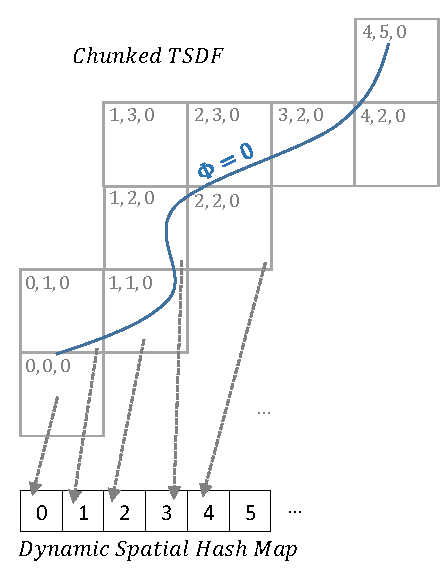
\includegraphics[width=1.0\textwidth]{img/chunks.pdf}
 	      \caption{Spatial Hashing.}
 	  	\label{fig:chunks} 
 	  \end{subfigure} 
 	  \begin{subfigure}[b]{0.55\linewidth} \centering
 	  	  \hspace{-5em}
	      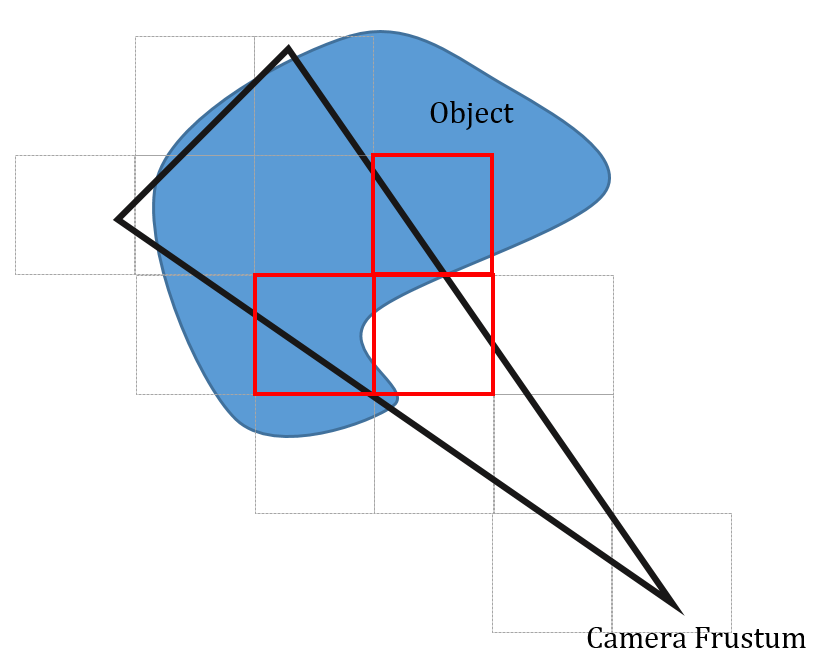
\includegraphics[width=1.0\textwidth]{img/frustum_cull}
	      \caption{Frustrum Culling.}
	 	 \label{fig:frustum_cull}
	  \end{subfigure}
	  \caption{\figref{fig:chunks}: chunks are spatially-hashed \cite{SpatialHashing} into a
      dynamic hash map. 
      \figref{fig:frustum_cull}: only voxels within the frustrum (in green) are stored in memory.}
\end{figure} 

Each voxel contains an estimate of the signed distance field and an
associated weight. In our implementation, these are packed into a single 32-bit
integer. The first 16 bits are a fixed-point signed distance value, and the
last 16 bits  are an unsigned integer weight. Color is similarly
stored as a 32 bit integer, with 8 bits per color channel, and an 8 bit weight.
A similar method is used in \cite{Newcombe, Whelan2013, Bylow2013, NiessnerHashing} to store
the \TSDF. As a baseline, we could consider simply storing all the required
voxels in a monolithic block of memory. Unfortunately, the amount of memory storage required
for a fixed grid of this type grows as $\mathcal{O}(N^3)$, where $N$ is the
number of voxels per side of the 3D voxel array. Additionally, if the size of
the scene isn't known beforehand, the memory block must be resized.

% For example, at a resolution of $3\text{cm}$,  a $30\text{m}$ TSDF cube
% with color would occupy 8 Gigabytes of memory. Worse, most of that memory would be
% uselessly storing unseen free space.

For a large-scale real-time suface reconstruction application, a less
memory-intensive and more dynamic approach is needed. Confronted with this
problem, some works have either used  octrees \cite{Wurm2010, Zeng2012,
Chen2012}, or use a moving volume\cite{Whelan2013}. Neither of these approaches
is desirable for our application. Octrees, while maximally memory efficient,
have significant drawbacks when it comes to accessing and iterating over the
volumetric data \cite{NiessnerHashing}. Every time an octree is queried,  a
logarithmic $\mathcal{O}(M)$ cost is incurred, where $M$ is the depth of the
Octree. In contrast, queries in a flat array are $\mathcal{O}(1)$. An octree
stores pointers to child octants in each parent octant. The octants themselves
may be dynamically allocated on the heap. Each traversal through the tree
requires $\mathcal{O}(M)$ heap pointer dereferences in the worst case.
Even worse, adjacent voxels may not be adjacent in memory, resulting in very
poor caching performance \cite{CacheStructures}.  Like \cite{NiessnerHashing},
we found that using an octree to store the \TSDF data to reduce iteration
performance by an order of magnitude when compared to a fixed grid.

\begin{figure*}[t!]
  \centering
	 \begin{subfigure}[b]{0.22\linewidth} \centering
			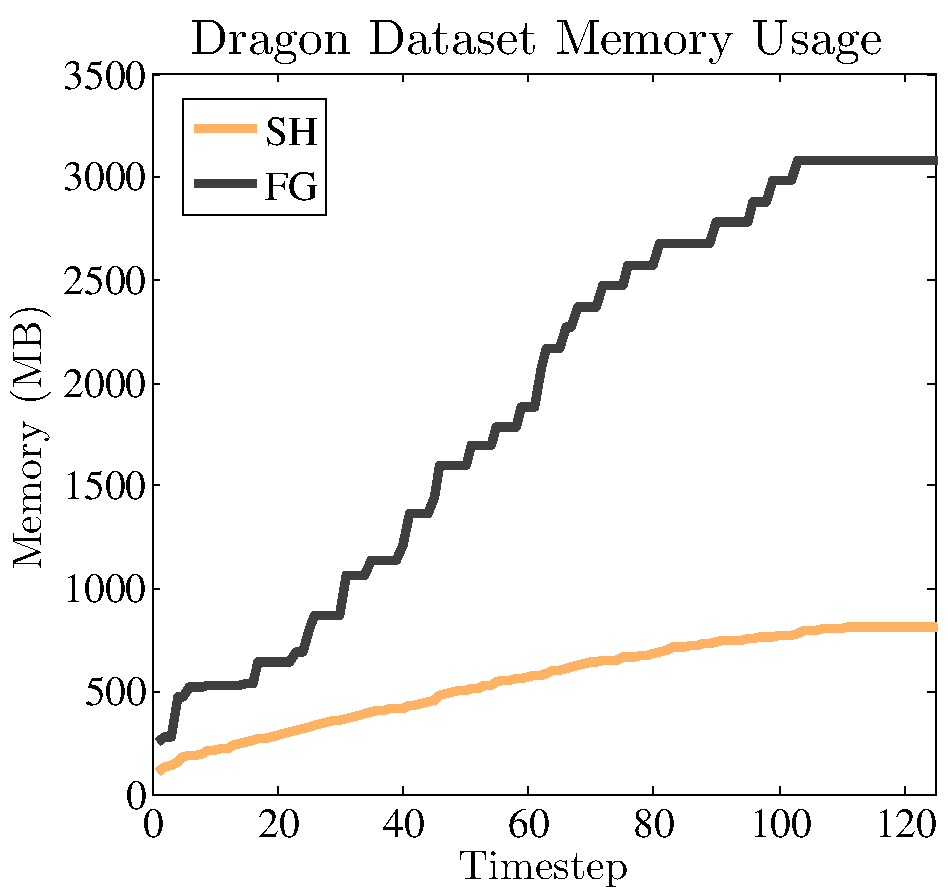
\includegraphics[width=1.0\textwidth]{img/memoryusage.pdf}
			 \caption{Memory usage efficiency.} 
			 \label{fig:memory_data}
		 \end{subfigure}  
		  \begin{subfigure}[b]{0.22\linewidth} \centering
			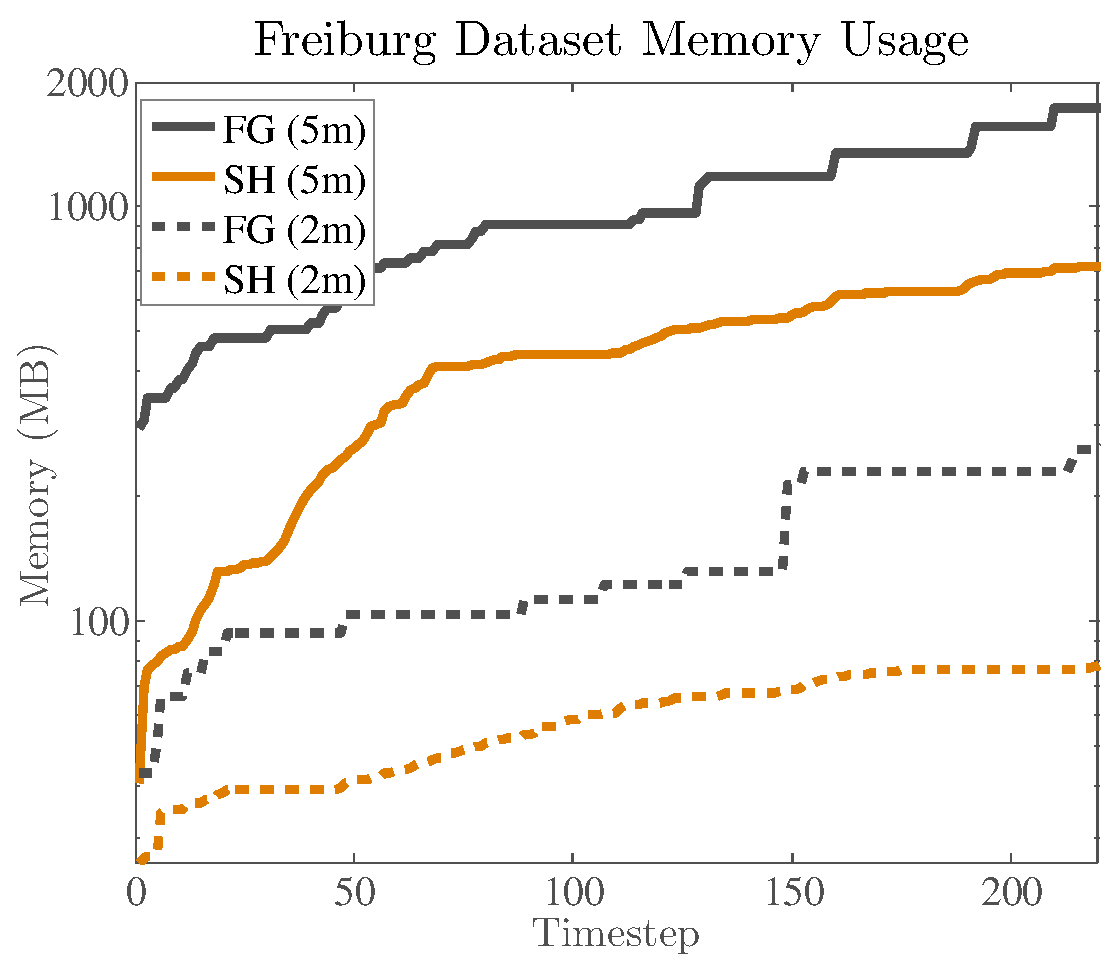
\includegraphics[width=1.0\textwidth]{img/memoryusage2.pdf}
			 \caption{Varying depth frustrum.} 
			 \label{fig:memory_data2}
		 \end{subfigure}
	  \begin{subfigure}[b]{0.27\linewidth} \centering 
		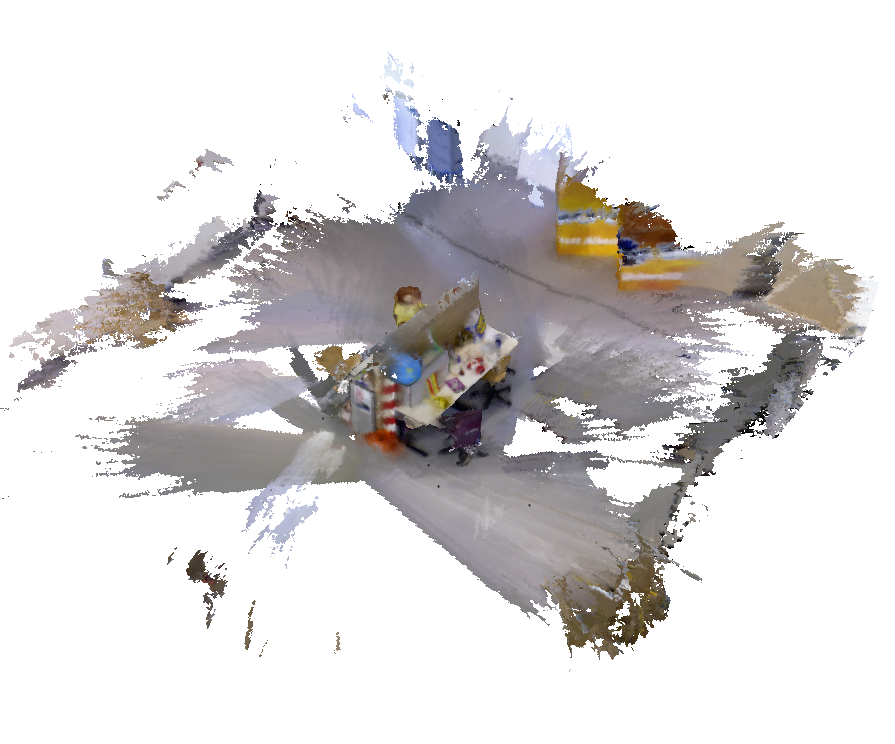
\includegraphics[width=1.0\textwidth]{img/freiburg_5m.png}
		 \caption{5m depth frustrum.}
		 \label{fig:freiburg_5m}
	 	\end{subfigure} 
 		\begin{subfigure}[b]{0.27\linewidth} \centering
		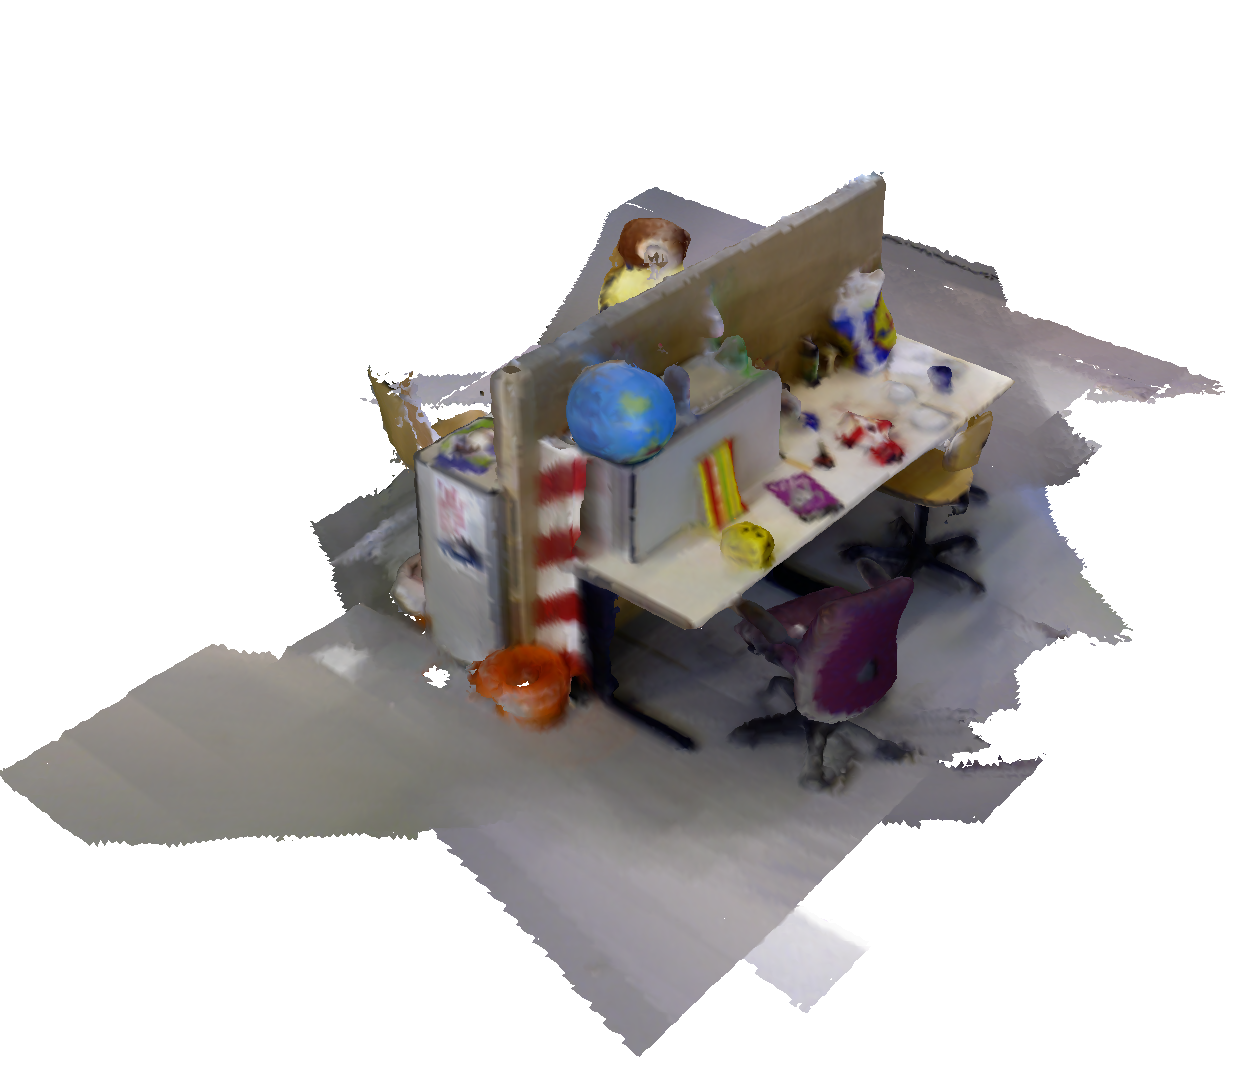
\includegraphics[width=1.0\textwidth]{img/freiburg_2m.png}
		 \caption{2m depth frustrum.} 
		 \label{fig:freiburg_2m}
	 \end{subfigure}
	 \caption{Spatial Hashing (SH) is more memory efficient than Fixed Grid (FG) and provides control over depth frustrum.}
\end{figure*} 

\begin{table}[t!]
\centering
	\begin{tabular} {rrr}
	\toprule
	Voxel Class & Voxel Count & \% of Bounding Box \\ 
	\midrule
	Unknown Culled & 62,105,216 & 77.0 \\ 
	Unknown & 12,538,559 & 15.5 \\ 
	Outside & 3,303,795 & 4.1 \\ 
	Inside & 2,708,430 & 3.4 \\ 
	\bottomrule
	\end{tabular}
	\caption{Voxel statistics for the Freiburg 5m dataset.}
	\label{table:volumecount}  
\end{table}

Instead of using an Octree, moving volume, or a fixed grid, we use a hybrid data
structure introduced by Niessner \etal \cite{NiessnerHashing}. We divide
the world into a two-level tree. In the first level we have \emph{chunks} of
voxels.  In \figref{fig:chunks}, voxel chunks (grey) are allocated near the
surface (blue) of the scene. Chunks are spatially-hashed \cite{SpatialHashing}
into a dynamic hash map.  Each chunk consists of a fixed grid of ${N_v}^3$
voxels, which are stored in a monolithic memory block. Chunks are allocated
dynamically from a growing pool of heap memory as data is added, and are
indexed in a spatial 3D hash map \cite{SpatialHashing} by their spatial
coordinates. As in \cite{SpatialHashing, NiessnerHashing} we use the hash
function:  $ \textbf{hash}(x, y, z) = p_1 x\oplus p_2 y \oplus p_3 z
~\text{mod}~n $, where $x, y, z$ are the 3D integer coordinates of the chunk,
$p_1, p_2, p_3$ are arbitrary large primes, $\oplus$ is the xor operator, and $n$ is
the maximum size of the hash map.

Since chunks are a fixed size, querying data from the chunked \TSDF involves
rounding (or bit-shifing, if $N_v$ is a power of two) a world coordinate to a
chunk and voxel coordinate, and then doing a hash-map lookup followed by an
array lookup. Hence, querying is $\mathcal{O}(1)$ \cite{NiessnerHashing}.
Further, since voxels within chunks are stored adjacent to one another in
memory, cache performance is improved while iterating through them. By carefully
selecting the size of chunks so that they corresponding to $\tau$, we only
allocate volumetric data near the zero isosurface, and do not waste as much
memory on empty or unknown voxels.

\subsection{Frustum Culling and Garbage Collection}
\label{section:frustum}
To determine which chunks should be updated by a depth scan and drawn, we use
frustum culling, a well known technique in computer graphics. We  create a
camera frustum with a far plane at the maximum depth reading of the camera, and
the near plane at the minimum depth of the camera. We then take the 
axis-aligned bounding box of the camera frustum, and check each chunk inside the
axis-aligned bounding box for intersection with the camera frustum. Only those
which intersect the frustum are updated.

Since the frustum is a conservative approximation of the space that could be
updated by a depth scan, some of the chunks that are visible to the frustum will
have no depth data associated with them. \figref{fig:frustum_cull} shows all the
\TSDF chunks which intersect the depth camera frustum and are within $\tau$ of
a hit as green cubes. Only these chunks are updated when new data is received. 
Chunks which do not get updated during a depth scan are garbage collected
(deleted from the hash map). Since the size of the camera frustum is in a fixed
range, the garbage collection process has $\mathcal{O}(1)$ performance. Niessner
\etal \cite{NiessnerHashing} use a similar approach for deciding which voxel
chunks should be updated using raycasting rather than geometric frustum
culling. We found frustum culling faster than raycasting on the mobile CPU.

\subsection{Depth Scan Fusion}
\label{section:scan_integration}
To fuse a depth scan into the \TSDF (\algoref{alg:TSDF}), it is necessary
to consider each depth reading in each scan and upate each
voxel intersecting its depth cone according to its distance to an observed
surface. The most straightfoward way of doing this is to simply step along
each cone, and then use a fast rasterization algorithm \cite{RayTracing} to determine which voxels
intersect with the cone. Most works  approximate the depth cone with a ray
through the center of the cone \cite{Newcombe, NiessnerHashing}. We will call
this the Raycasting approach. However, has performance bound by
$\mathcal{O}(N_{\text{ray}} \times l_{\text{ray}})$, where $N_{\text{ray}}$ is
the number of rays in a scan, and $l_{\text{ray}}$  is proportional to the
length of a ray being integrated. If we use a fixed-size truncation distance
and do not perform space carving, $l_{\text{ray}} = \tau$.
However, with space-carving (\sref{section:carving}), the length of a ray
being integrated is potentially unbounded.

A useful approximation of raycasting is \textit{projection mapping}. Used in
\cite{Newcombe,Nguyen2012, Bylow2013, Klingensmith2014}, projection mapping
works by projecting the visual hull of each voxel onto the depth image and
comparing the depth value there with the geometric distance from the voxel to
the camera plane. \algoref{alg:projection_mapping} describes projection mapping.
Instead of iterating over each ray, projection mapping iterates over each voxel.
Like most other works, we approximate each voxel's visual hull by a single point
at the center of the voxel.

Projection mapping has performance bounded by $\mathcal{O}(N_v)$, where $N_v$ is
the number of voxels affected by a depth scan. This value is nearly constant
over time, and depending on the resolution of the \TSDF, may be significantly
less than the number of rays in a scan. However, projection mapping suffers from
resolution-dependant aliasing errors, because the distance to the center of a
voxel may differ from the true length of the ray passing through the voxel by up
to the length of the diagonal of the voxel. Further, by ignoring the visual
hull of the voxel and only projecting its center, we ignore the fact that
multiple depth cones may intersect a voxel during each scan.
\sref{section:scan_compare} compares the performance and quality of these methods.

\begin{algorithm} 
	\caption{Projection Mapping}
	\label{alg:projection_mapping}
	\begin{algorithmic}[1]
		\For {$\mathbf{v}_c \in V$} \Comment{For each voxel}
		\State {$z \gets   \|\mathbf{o}_t - \mathbf{v}_c\|$}
		\State{$z_p \gets \mathbf{InterpolateDepth}(\mathbf{Project}(\mathbf{v}_c))$}
		\State{$u \gets z_p - z$} 
		\State{$\tau \gets \mathcal{T} (z_p)$}  \Comment{Dynamic truncation}
	    \If{$u \in [\tau + \epsilon, z_p]$} \Comment{Space carving region}
	    	\If {$\Phi_{\tau}(\mathbf{v}_c) \leq 0$ }
		    	\State {$\Phi_{\tau}(\mathbf{v}_c) \gets \text{undefined}$}
		    	\label{alg:line:voxel_carve}
				\State {$W(\mathbf{v}_c) \gets 0$}
			\EndIf
	    \EndIf
		\If{$u \in [-\tau, \tau]$}  \Comment{Hit region}
			\State {$\Phi_{\tau}(\mathbf{v}_c) \gets \frac{ W(\mathbf{v}_c)
			\Phi_{\tau}(\mathbf{v}_c)+ \alpha(u) u}{W(\mathbf{v}_c) +\alpha(u)}$}
			\label{alg:line:tsdf_update}
			\State {$W(\mathbf{v}_c) \gets W(\mathbf{v}_c)+ \alpha(u)$}
		\EndIf
	\EndFor
	\end{algorithmic}
\end{algorithm}
\subsection{Rendering}
\label{section:render}
Most other \TSDF fusion methods \cite{Newcombe, NiessnerHashing} render the
scene by directly raytracing it on the GPU. Hardware limitations prevent us from doing
this. Instead, we use an approach from computer graphics for rendering large
terrains \cite{GPUGEMS3} using incremental Marching Cubes \cite{Lorensen1987}.
For each chunk, we store a triangle mesh. Meshing is done asynchronously with
the depth scan fusion, and is performed lazily (\ie, only when chunks need to
be rendered).

Triangle meshes are generated at the zero isosurface whenever the chunk has been
updated by a depth scan. As in \cite{Bylow2013, Whelan2013},  colors are
computed for each vertex by trilinear interpolation. At the borders of chunks,
vertices are duplicated. Only those meshes which are visible to the virtual camera
frustum are rendered. Meshes that are very far away from the camera are
rendered as a colored bounding box. Meshes far away from the virtual camera are
destroyed once the number of allocated meshes exceeds some threshold.

\subsection{Pose Estimation}
\label{section:pose}
We assume we  have \textit{a priori} black-box pose estimation of the
sensor from a seperate pose tracking system. Specifically, in our experiments,
pose data is estimated from an onboard visual-inertial odometry system that fuses
data from a wide-angle camera, an inertial measurement unit, and a gyroscope at
60 Hz using 2D feature tracking and an Extended Kalman Filter. A more detailed
discussion of this system can be found in \cite{VINS, VINS2}.  Unlike
most other \TSDF fusion methods \cite{Newcombe, Whelan2013,
Bylow2013, NiessnerHashing} , our implementation makes no attempt to estimate
the pose of the sensor directly from depth data. Instead, we use depth data 
only for surface reconstruction. Unfortunately, decoupling the pose estimation
and surface reconstruction results in failure to correct for drift in the pose
estimation using depth data, and can result in mis-alignment of depth scans
\figref{fig:drift} shows a top down view of a $\sim
175$ meter long corridor reconstructed by a user holding the device. The
left figure shows the reconstruction achieved by visual odometry alone,
with $\sim 5$ meter drift present at the end of the corridor. The right 
figure shows the reconstruction after the trajectory has been globally
optimized offline using bundle adjustment, overlaid on the floorplan of
 the building. We found that using direct scan-to-model ICP (as in
 \cite{Newcombe}) to augment visual odometry and sparse keypoint mapping to be
 too slow to run in real-time on the device along with \TSDF fusion. This is not
 to say that another approach combining sparse keypoints with occlusion data
 from the \TSDF (as in \cite{StuecklerSparseDense}), would not work.

% Section removed to save space
% \subsubsection{Pose Interpolation}
% We will assume that pose estimation, depth sensing, and color sensing are
% asynchronously executed, so we may not have all three measurements at a given
% time. To deal with asynchronous sensing and pose estimation, we linearly
% interpolate poses over time to determine the pose of a given sensor at any given time.
% 
% Call the global pose estimate of the sensor at time $t$,  ${H_{s}}^t$.
% Additionally, assume we have apriori extrinsic pose estimates for the color
% sensor ${E_{c}}$ and the depth sensor ${E_{d}}$. We are given a discrete
% trajectory of pose estimates from the visual-inertial odometry system:
% 
% $$ {H_{s}}^{t_1}, {H_{s}}^{t_2}, \ldots, {H_{s}}^{t_T} $$
% 
% Suppose at time $t'$, we get a color image. Assume that $t'$ is not represented
% in the list of sensor body poses. Then, either $t' < t_1$,  $t' > t_T$, or
% $t_a < t < t_b'$ for some $a, b \in [1, T]$. In the first case ($t' < t_1$), we
% disregard the color image. In the second case ($t' > t_T$), we wait until more data is
% acquired. In the third case, we would interpolate the pose of the color camera
% as:
% 
% $$ {H_{c}}^{t'} \approx E_c \cdot \textbf{Interp}\left(H_{s}^{t_a}, H_{s}^{t_b},
% \frac{t' - t_a}{t_b - t_a}\right) $$
% 
% Where $\textbf{Interp}$ is a function that  interpolates between two
% poses by linearly interpolating translation while spherically interpolating
% rotation, using $\frac{t' - t_a}{t_b - t_a} \in [0, 1]$ as an interpolation
% parameter. 

% Section removed to save space
% \subsection{User Interface}
% We developed a simple and intuitive prototype interface to test our approach on
% the device. Users were presented with options for controlling the resolution of
% the reconstruction, and were able to control when the system was active and
% inactive, allowing them to pause when moving objects obscured objects they were
% trying to model.
% 
% We present the user with camera controls as well. A virtual first person
% camera mimics the intrinsics of the depth camera. A third-person camera allows
% the user to rotate the virtual camera around their current position and get a
% better look at the quality of the reconstruction; and an orthographic overhead
% camera functions as a global map of where the user has been (Figure
% \ref{fig:map_device}).
% 
% At any time, the user can save the volumetric representation of the TSDF, or a
% surface mesh generated by marching cubes to disk. 

 \begin{figure} [t!]\centering
		 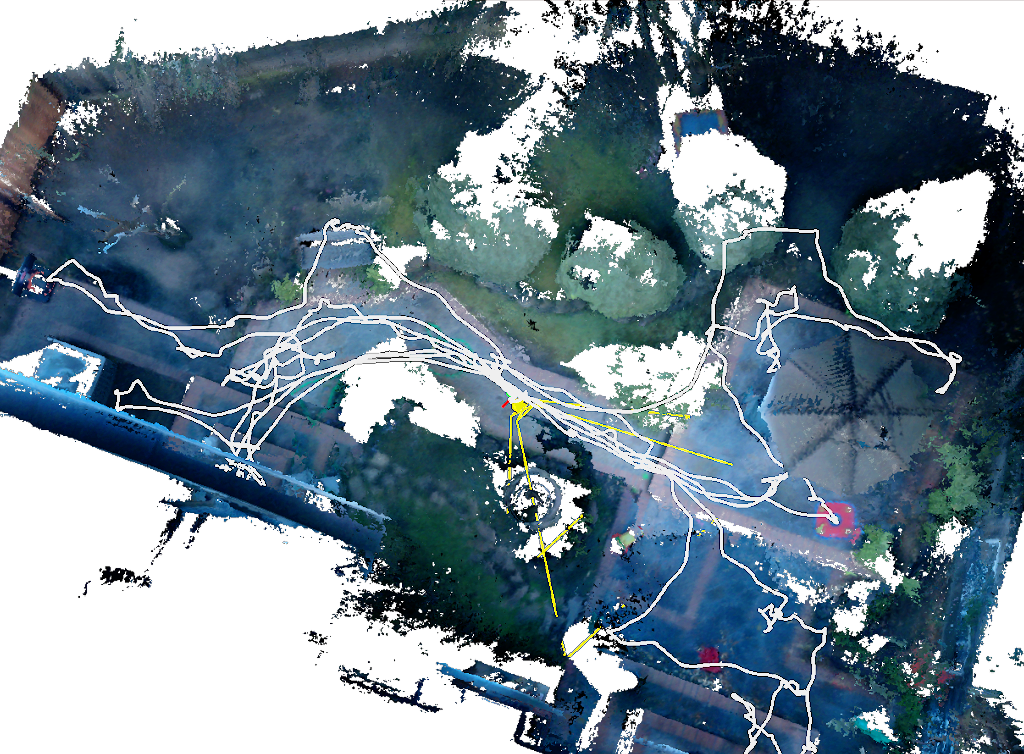
\includegraphics[width=0.9\linewidth]{img/colorbalance3}
		 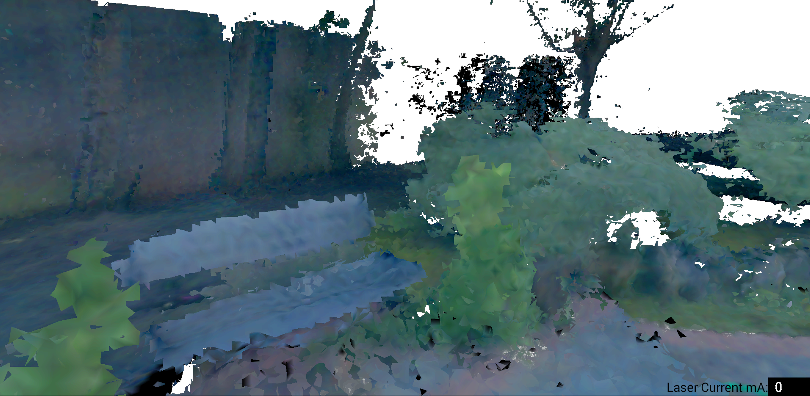
\includegraphics[width=0.45\linewidth]{img/colorbalance2}
		 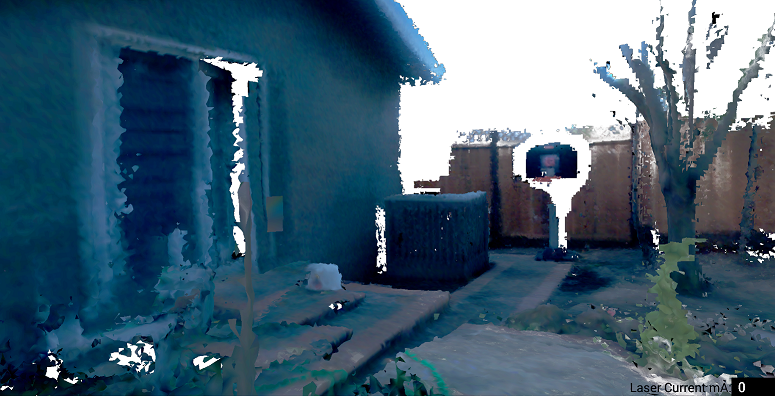
\includegraphics[width=0.45\linewidth]{img/colorbalance1} 
		 \caption{Outdoor scene reconstruction.}
		 \label{fig:night3}
\end{figure}

 \begin{figure*} [htb]\centering
	 	 \begin{subfigure}[b] {0.25\linewidth} \centering
		 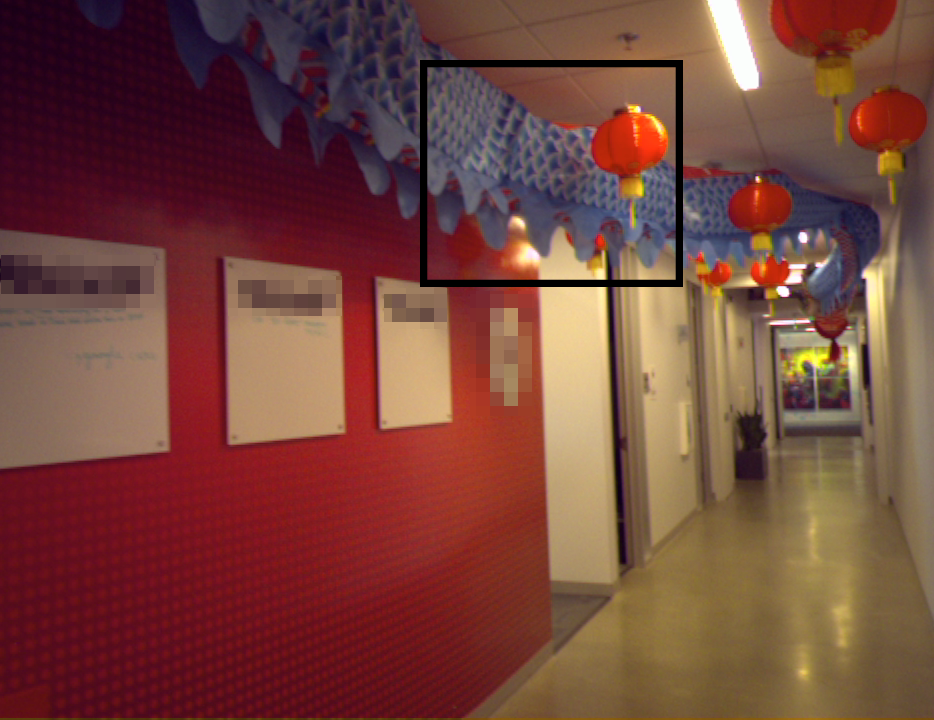
\includegraphics[width=1.0\textwidth]{img/dragon_color.png}  
		 \caption{A 15 meter hallway.}
		 \label{fig:dragon_color}
	 \end{subfigure}
	 	 \begin{subfigure}[b]{0.285\linewidth} \centering  
		 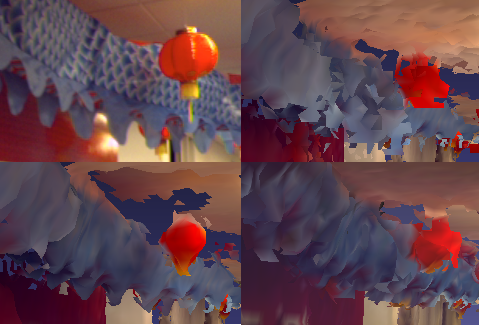
\includegraphics[width=1.0\textwidth]{img/dragon_closeup.png} 
		 \caption{Comparison of fusion techniques.}
		 \label{fig:dragon_closeup}
	 \end{subfigure} 
 	  \begin{subtable}[b]{0.4\linewidth} \centering
	\newcommand{\no}{{\ensuremath{\times}}}
	\newcommand{\yes}{{\ensuremath{\checkmark}}}
	\resizebox{\linewidth}{!}{
	\begin{tabular} { ccccc}
	\toprule
	Method       & Color & Carving & Desktop (ms.) & Tablet (ms.)\\
	\midrule 
	\multirow{4}{*}{Raycast} & \no & \no &$\mathbf{14 \pm 02}$ & $\mathbf{62 \pm 13}$ \\ 
	 & \yes & \no & $\mathbf{20 \pm 05}$ & $\mathbf{80 \pm 16}$ \\ 
	 & \no & \yes & $53 \pm  10$ & $184 \pm 40$ \\ 
	 & \yes & \yes &$58 \pm 16$  & $200 \pm 37$\\ 
	\midrule
	\multirow{4}{*}{Project} & \no & \no & $33 \pm 05$ & $106 \pm 22$ \\ 
	 & \yes & \no & $39 \pm 05$  & $125 \pm 23$ \\ 
	 & \no & \yes & $\mathbf{34 \pm 04}$  & $\mathbf{116 \pm 19}$ \\ 
	 & \yes & \yes  & $\mathbf{40 \pm 05}$ & $\mathbf{128 \pm 24}$ \\ 
	\bottomrule
	\end{tabular}
	}
			\caption{Single scan fusion time.}
			\label{table:timing}
	 \end{subtable} 
	 \caption{\figref{fig:dragon_closeup} is a closeup of
	 \figref{fig:dragon_color}.
	 Counter-clockwise from the top left: color image, projection mapping without
	 space carving, projection mapping with space carving, and raycasting without
	 space carving. \figref{table:timing} reports timing results.}
	 \label{fig:device_data}
 \end{figure*} 

\section{Experiments and Results}
\label{section:experiments}
\subsection{Hardware}
\label{section:hardware}
We implemented \chisel on two devices: a \Tango
``Yellowstone" tablet device, and a \Tango ``Peanut'' mobile 
phone device. The phone device has 2GB of RAM, a quadcore
CPU, a six-axis gyroscope and accelerometer, a wide-angle $120^\circ$ field of
view tracking camera which refreshes at 60Hz, a projective depth sensor which
refreshes at 6Hz, and a 4 megapixel color sensor which refreshes at 30Hz. The
tablet device has 4GB of ram, a quadcore CPU, an Nvidia Tegra K1 graphics card,
an identical tracking camera to the phone device, a projective depth sensor
which refreshes at 3Hz, and a 4 megapixel color sensor which refreshes at 30Hz.
%Devices were depth calibrated \ref{subsection:calibration} prior to testing. 

%  \subsection{Sensor Calibration}
% \label{subsection:calibration}
% The depth image may be corrupted by noise, feature nonlinear distortions, and
% have large segments of missing data. Our noise model of the sensor will consider
% Gaussian noise on the depth, and per-pixel quadratic distortion. Call a
% particular depth reading from the device the random variable $D$, and the true
% depth of the scene at that point $z$. Then we have the model:
%  
%  \begin{equation}
%  	D = z + a{z}^2 + b z + c+ \epsilon(z)
%  	\label{eqn:distort}
%  \end{equation} 
%  
%  \noindent where $a, b, c$ are coefficients of a quadratic depth distortion
%  model, and $\epsilon(z)$ is a random variable drawn from the parametric
%  Gaussian distribution function $\mathcal{N}(z, \sigma(z))$.
%  That is, the distribution is mean-centered on $z$, and has a depth-dependant
%  standard deviation $\sigma(z)$.
%  
%  We have found that on the \textit{Tango}  Peanut \cite{Tango} device, the
%  nonlinear distortion is very severe. At a distance of 3 meters, the reading
%  can be distorted by as much as 30 centimeters. Depth distortion on the
%  Yellowstone device is comparably negligible.  To get an accurate
%  reconstruction of the world, it is critical to correct for this distortion.
%  This is done by inverting the distortion model (\eref{eqn:distort}) to
%  estimate the true depth $z$ from the distorted reading $D$.
%   
%  \begin{figure} \centering
% 	 \begin{subfigure} {0.3\columnwidth} \centering
% 		 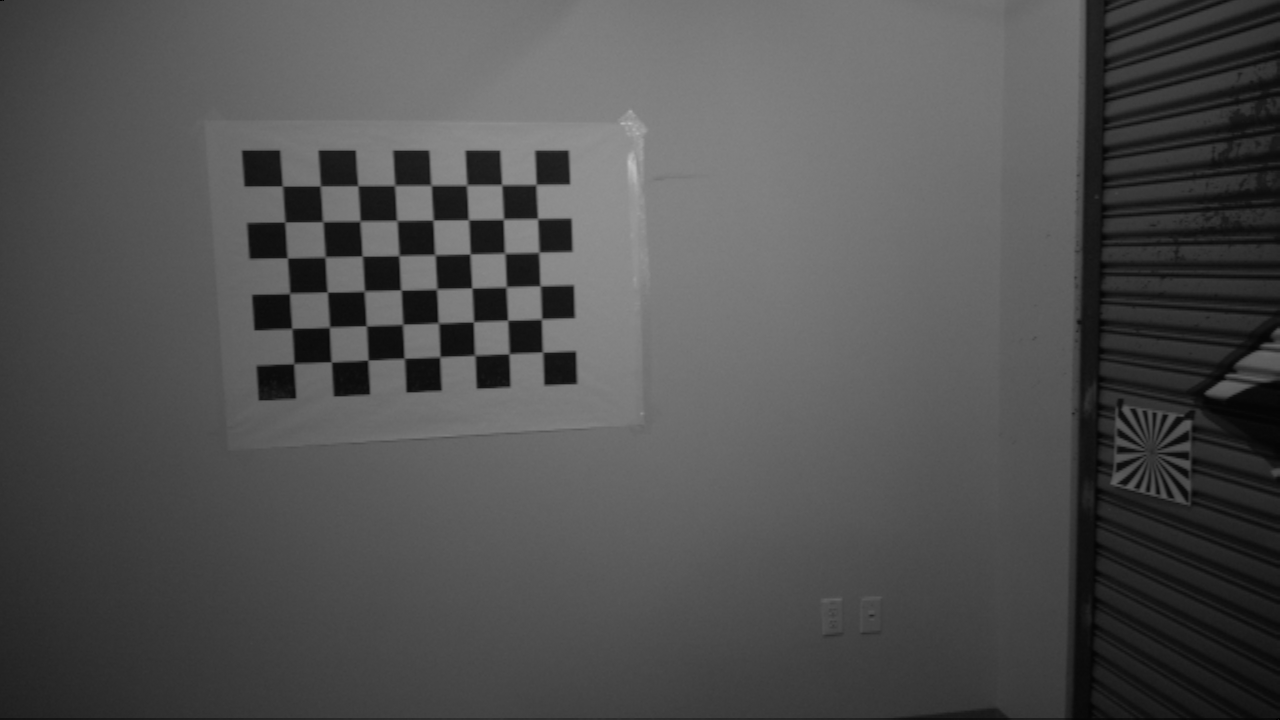
\includegraphics[width=1.0\textwidth]{img/calibration_grey}
% 		 \caption{}
% 	 \end{subfigure}
% 	 \begin{subfigure}{0.3\columnwidth} \centering
% 		 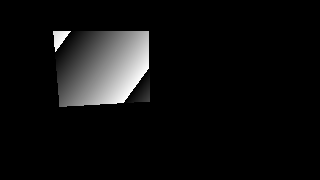
\includegraphics[width=1.0\textwidth]{img/calibration_model}
% 		 \caption{}
% 	 \end{subfigure}
% 	 	 \begin{subfigure}{0.3\columnwidth} \centering
% 		 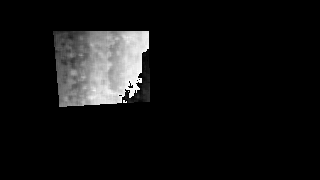
\includegraphics[width=1.0\textwidth]{img/calibration_data}
% 		 \caption{}
% 	 \end{subfigure}
% 	 \caption{Components collected in our calibration procedure. The greyscale (a)
% 	 image is used to compute a linear plane model (b) for depth. That model is
% 	 compared to the actual depth data (c) over a series of checkerboard poses.}
% 	 \label{fig:calibration}
%  \end{figure}
%  
%  To train the distortion and noise model, we first calibrate the sensor with the
%  use of a checkerboard calibration target. Images of the target are taken at
%  multiple distances and angles from the camera (\figref{fig:calibration}). We
%  fit an ideal plane to the target to determine what the true distance should be
%  at each pixel. Then, we perform quadratic regression on the depth readings
%  against the predicted readings from the plane to find the per-pixel distortion
%  coefficients. The function $\sigma(z)$ is computed in a similar way, by
%  computing a histogram of standard deviations of the depth readings, and then
%  performing quadratic regression on the result. A single function $\sigma(z)$ is used for the
%  entire image, unlike the distortion model which is computed on a per-pixel
%  basis.
%  
\subsection{Use Case: House Scale Online Mapping}
\label{section:mapping}
Using our system, we are able to create and display large scale maps at a
resolution as small as 2cm in real-time on board the device.
\figref{fig:map_device} shows a map of an office building floor being
reconstructed in real-time using the phone device.  This scenario is also shown
in a video here \cite{VIDEO}. \figref{fig:drift} shows a similar reconstruction
of a $\sim 175m$ office corridor. Using the tablet device, we have reconstructed
(night time) outdoor scenes in real-time.\figref{fig:night3} shows an outdoor scene
captured at night with the yellowstone device at a 3cm resolution. The yellow
pyramid represents the depth camera frustum. The white lines show the trajectory
of the device.

In the course of online mapping, the user has immediate feedback on model
completeness, and can pause mapping for live inspection. The system continues
localizing the device using visual-inertial odometry even when the mapping is
paused. After mapping is complete, the user can save the map to disk.
 
 \subsection{Use Case: Aerial Robot Motion Planning}
 \label{section:robot}
  \begin{figure}
  \centering
   	 \begin{subfigure}{0.55\columnwidth}\centering
 	 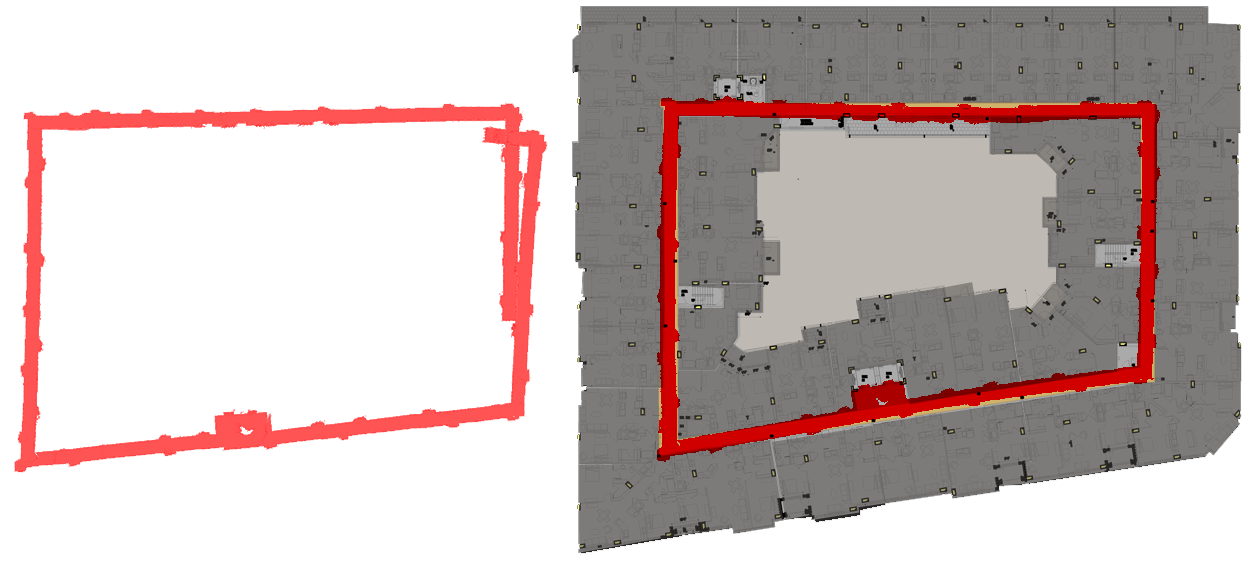
\includegraphics[width=1\textwidth]{img/corridor_composite.png}
 	 \caption{System pose drift in a long corridor.}
 	 \label{fig:drift}
 	 \end{subfigure}
  \begin{subfigure}{0.43\columnwidth}\centering
	 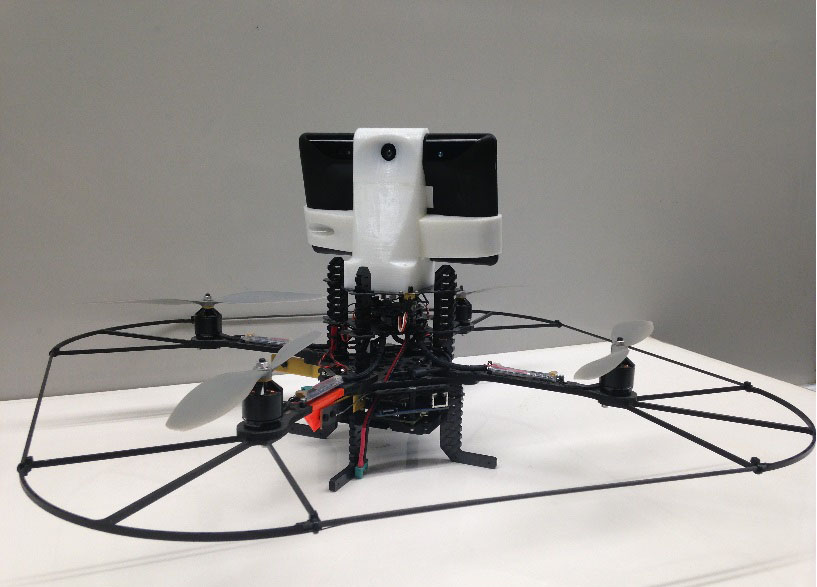
\includegraphics[width=1.0\textwidth]{img/aerial.jpg}
	 \caption{An aerial robot with a tablet device attached.}
	 \label{fig:robot}
  \end{subfigure}
	\begin{subfigure}{0.8\columnwidth}\centering
	 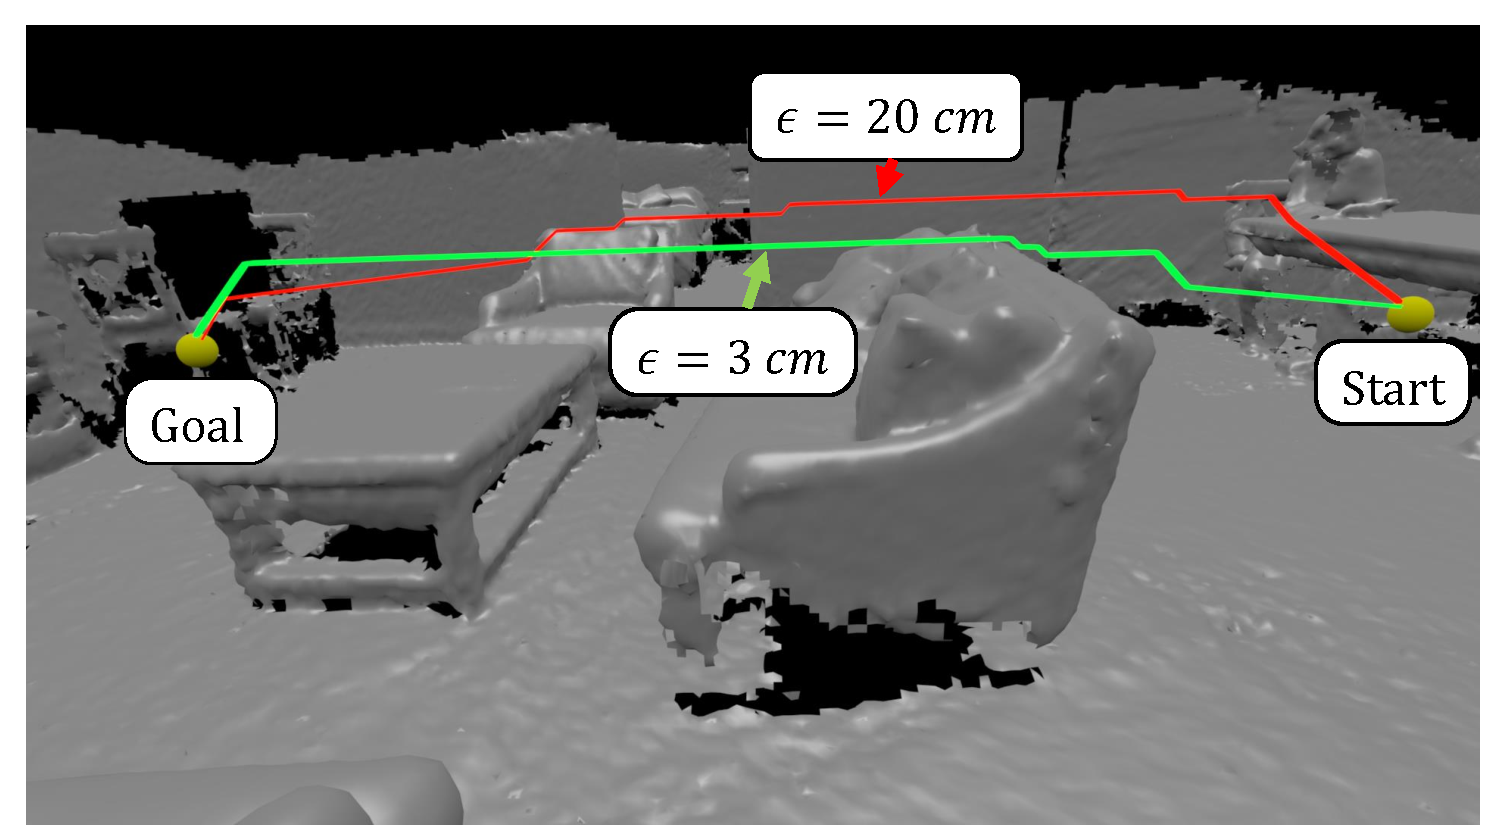
\includegraphics[width=1\textwidth]{img/path_plan.pdf}
	 \caption{A 3D motion plan through the \TSDF}
	 \label{fig:path_plan}
	 \end{subfigure}
      \caption{}
  \label{fig:robot_figure}
\end{figure} 
 One of the main advantages of fully-integrated hardware systems such as the
\Tango device is that they are light enough to mount on small mobile
 robots. As a motivating example, consider the problem of motion planning in
 a scene created onboard the device using \chisel. \figref{fig:robot} shows a
 robot on which we mounted a tablet device. The device is light enough to allow
 the robot to fly.
 
 As in \cite{FlyingNavigation}, we simulate a motion planning problem for an
 aerial robot by planning for a sphere-shaped robot in 3D. Note that a sphere-shaped robot can be
 represented as a point when planning in a distance field. The distance to the
 nearest surface for a robot with radius $\epsilon$ is $d_{\epsilon}(x) =
 \Phi_\tau(x) - \epsilon$. We want to find a 3D trajectory $\xi$ which
 minimizes:
 
 \begin{equation}
      c_{\epsilon}(\xi) = a \sum_{x \in \xi} \left(\tau -
      d_{\epsilon}(x)\right) + b\|\xi\|_2
 \end{equation} 
 
\noindent where $\|\xi\|_2$ is the length of the trajectory, and $a, b$ are
positive weights. This can be accomplished using the A* algorithm on a
26-conntected lattice grid, with a simple Euclidean heuristic function. Note
that the edge weights are garunteed to be positive (because all distances in the
\TSDF are $\leq\tau$). Whenever $d < 0$, the robot is considered to be in
collision, and no expansions are made.
\figref{fig:path_plan} shows two example paths through a pre-scanned \TSDF scene.
Notice that by varying $\epsilon$, trajectories can be made to skirt closer or further from obstacles without
additional computation cost.
 
\subsection{Comparing Depth Scan Fusion Algorithms} 
\label{section:scan_compare}
We implemented both the raycasting and voxel projection modes of depth scan
fusion (\sref{section:scan_integration}), and compared them in terms of speed
and quality. \tabref{table:timing} shows timing data for different scan
insertion methods is shown for the ``Room'' dataset
(\figref{fig:apartment_color}) in milliseconds. Raycasting (\algoref{alg:TSDF})
is compared with Projection Mapping (\algoref{alg:projection_mapping}) on both a
desktop machine and a \Tango tablet. Results are shown with and without
space carving (\sref{section:carving}) and colorization
(\sref{section:color}).The fastest method in each category is shown in bold. We
found that projection mapping was far more efficient than raycasting when space
carving was used. However, projection mapping results undesirable aliasing
artifacts; especially on surfaces nearly parallel with the camera's visual axis.
Additionally, color consistency suffers with projection carving, because rather
than color being averaged by all the rays passing through each voxel, only a
single color is used for each projected voxel center. The use of space carving
drastically reduces noise artifacts, especially around the silhouettes of
objects (\figref{fig:dragon_closeup}). We note that using both space carving
\emph{and} raycasting is not fast enough for real-time mapping on the device
using our system.

\begin{table}
\centering
\begin{tabular} {rr@{ $\pm$ }lr@{ $\pm$ }l} \toprule
\TSDF Method & \multicolumn{2}{c}{Meshing Time (ms.)} & \multicolumn{2}{c}{Update Time (ms.)}\\ 
\midrule
$256^3$ Fixed Grid     & 2067 & 679 & 3769 & 1279  \\
$16^3$ Spatial Hashing & 102  &  25 & 128 &   24   \\ 
\bottomrule
\end{tabular}
\caption{The time taken per frame in milliseconds to generate meshes
(\sref{section:render}), and update the \TSDF using colorization, space carving, and projection mapping
are shown for the ``Room'' (\figref{fig:apartment_color}) dataset.}
\label{table:meshingtimes}
\end{table}

\subsection{Memory Usage}
\label{section:memory}

\tabref{table:volumecount} shows voxel statistics for the Freiburg 5m
(\figref{fig:freiburg_5m}) dataset. Culled voxels are not stored in  memory.
Unknown voxels have a weight of 0. Inside and Outside voxels have a weight $>
0$ and an SDF than is $\leq 0$ and $> 0$ respectively. Measuring the amount of
space in the bounding box that is culled, stored in chunks as unknown, and
stored as known, we found that the vast majority (77\%) of space is culled, and
of the space that is actually stored in chunks, 67.6\% is unknown. This fact
drives the memory savings we get from using the spatial hashmap
technique from Niessner \etal \cite{NiessnerHashing}.

We compared memory usage statistics of the dynamic spatial hashmap (SH) to
a \naive fixed-grid data structure (FG) which allocates a single block of memory to
tightly fit the entire volume explored (\figref{fig:memory_data}). As the size of the space
explored increases,  spatial hashing  with $16 \times 16 \times
16$ chunks uses about a tenth as much memory as the fixed grid algorithm. Notice
that in \figref{fig:memory_data}, the \naive data structure uses nearly 300MB of RAM 
whereas the spatial hashing data structure never allocates more than 47MB of RAM
for the entire scene, which is a 15 meter long hallway.

We tested the spatial hashing data structure (SH) on the publicly available Freiburg
RGB-D dataset \cite{FREIBURG}, which contains ground truth pose information from a motion
capture system (\figref{fig:freiburg_2m}). In the Freiburg office dataset, a
\textit{Kinect} sensor makes a loop around a central desk scene. The room is
roughly 12 by 12 meters in area.  Memory usage statistics (Fig.
\ref{fig:memory_data2}) reveal that when all of the depth data is used
(including very far away data from the surrounding walls), a \naive fixed grid
data structure (FG) would use nearly 2GB of memory at a 2cm resolution, whereas
spatial hashing with $16 \times 16 \times 16$ chunks uses only around 700MB.
When the depth frustum is cut off at 2 meters (mapping only the desk structure
without the surrounding room), spatial hashing uses only 50MB of memory, whereas
the \naive data structure would use nearly 300MB. We also found that running marching
cubes on a fixed grid rather than incrementally on spatially-hashed chunks
(\sref{section:render}) to be prohibitively slow (\tabref{table:meshingtimes}). 

% \begin{table}
% \footnotesize
% \hfill
% \centering
% \begin{tabular} {| l | r | r |}
% \hline
% Voxel Class & Voxel Count & \% of Bounding Box \\ \hline
% Unknown Culled & 62,105,216 & 77.0\% \\ \hline
% Unknown & 12,538,559 & 15.5\% \\ \hline
% Outside & 3,303,795 & 4.1\% \\ \hline
% Inside & 2,708,430 & 3.4\% \\ \hline
% \end{tabular}
% \caption{Voxel statistics for the Freiburg (\figref{fig:freiburg_5m}) dataset.
% $16\times16\times16$ chunks are allocated at a 2cm resolution. Culled voxels are
% not stored in memory. Unknown voxels have a weight of 0. Inside and Outside
% voxels have a weight $> 0$ and an SDF than is $\leq 0$ and $> 0$ respectively. }
% \label{table:volumecount}
% \end{table} 

% \subsection{Limitations due to Odometry Drift}
% Since we do not update pose using depth data, odometry pose drift severely 
% corrupts the map, especially when the same area is repeatedly scanned . We  
% compare the map produced online using visual-inertial odometry to one produced
% offline by first correcting the pose of the camera using bundle adjustment (a
% process which takes several hours) to show the effect of drift  (Figure
% \ref{fig:bundleadjust}). Double walls, accidentally carved space, and other
% artifacts result when drift is present. Clearly, this limitation presents the
% need for dense loop closure and alignment. high-quality meshes produced using
% offline bundle adjustment for pose estimates are shown in figure
% (\ref{fig:apartment}).
% 
%   \begin{figure*} \centering
% 	 \begin{subfigure} {0.49\columnwidth} \centering
% 		 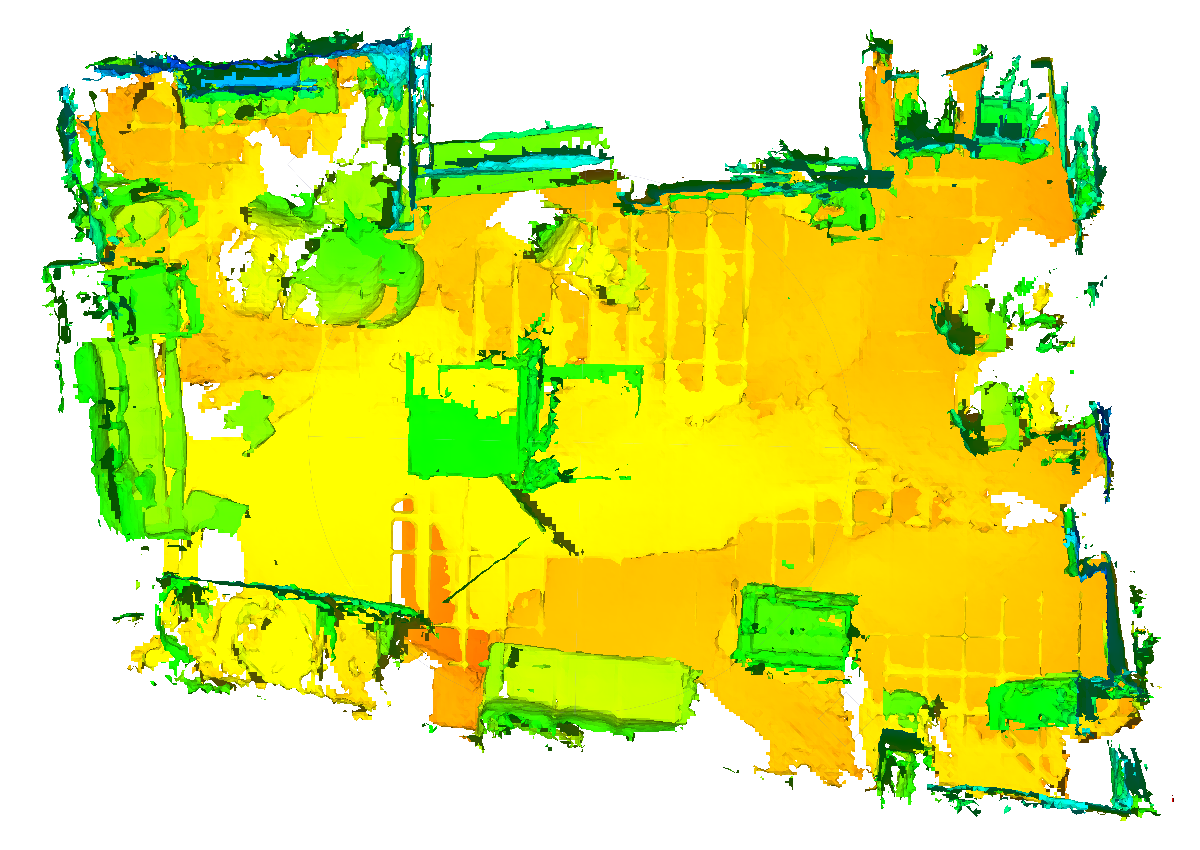
\includegraphics[width=1\textwidth]{img/gameroom_vio.png}  
% 		 \caption{}
% 		 \label{fig:gameroom_vio}
% 	 \end{subfigure}
% 	 \begin{subfigure}{0.49\columnwidth} \centering
% 		 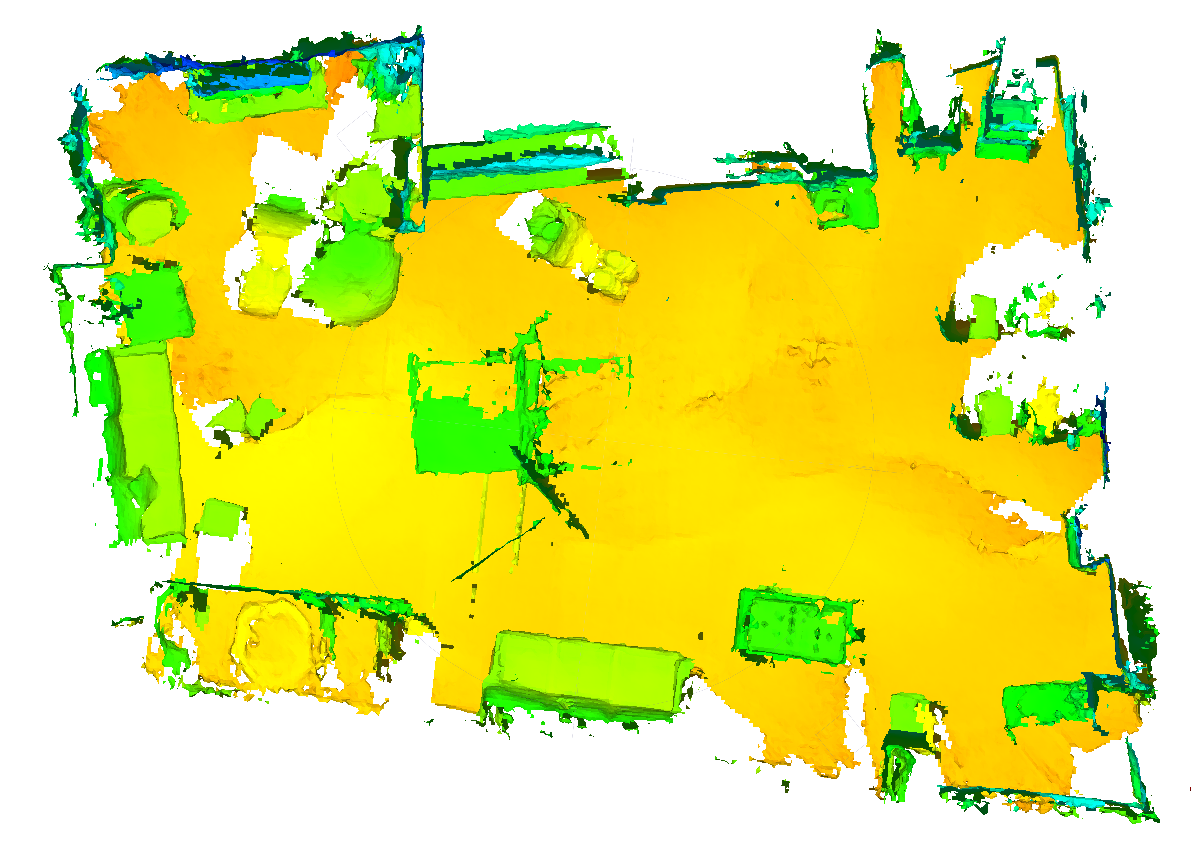
\includegraphics[width=1\textwidth]{img/gameroom_bundleadjust.png}
% 		 \caption{}
% 		 \label{fig:gameroom_bundleadjust}
% 	 \end{subfigure}
% 	 \caption{The phone device was used to scan a midsized room by walking in a
% 	 loop around the room three times. A top down view is shown. Meshes are colored
% 	 with respect to their height; the floor is orange and objects green. Drift
% 	 from visual-inertial odometry causes severe corruption and artifacts in the 
% 	 TSDF (\ref{fig:gameroom_vio}). By pre-processing the trajectory offline using
% 	 bundle adjustment, we can produce a much higher quality mesh using the same
% 	 dataset (\ref{fig:gameroom_bundleadjust}). Meshes are produced using
% 	 raycasting and space carving. }
% 	 \label{fig:bundleadjust}
%  \end{figure*}  
%  
%    \begin{figure*} \centering
% 	 \begin{subfigure} {0.49\columnwidth} \centering
% 		 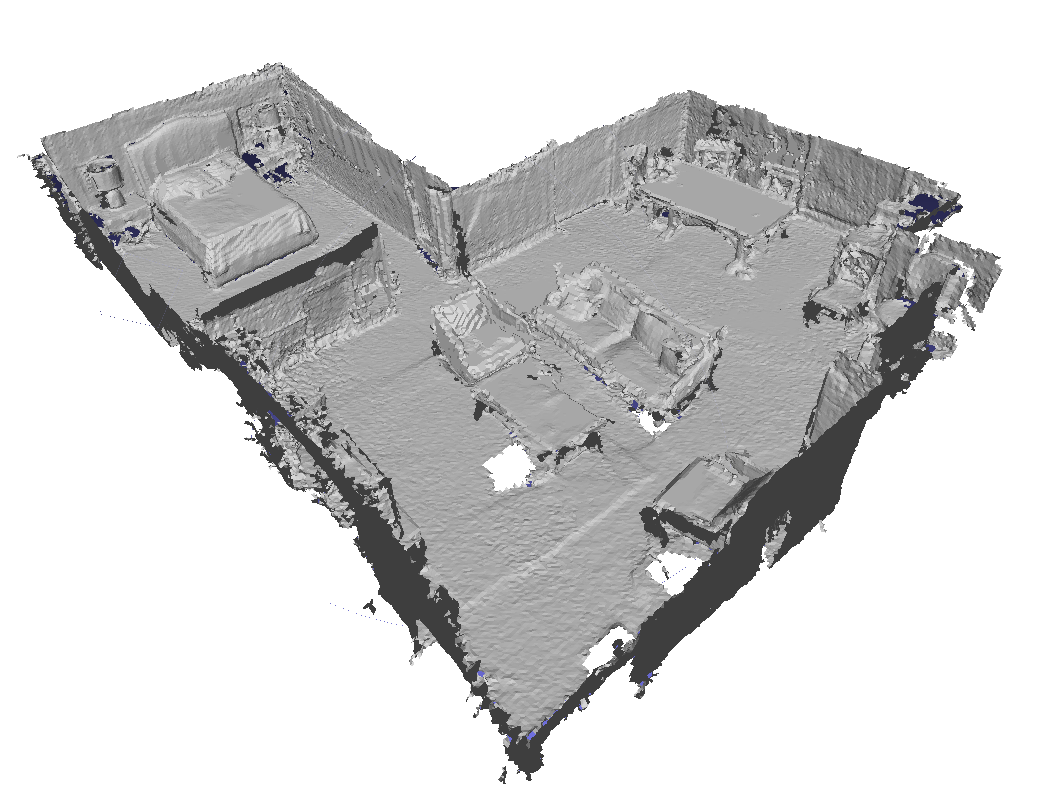
\includegraphics[width=1\textwidth]{img/apartment_scene_nocolor.png}  
% 		 \caption{}
% 		 \label{fig:aparment_nocolor}
% 	 \end{subfigure}
% 	 \begin{subfigure}{0.49\columnwidth} \centering
% 		 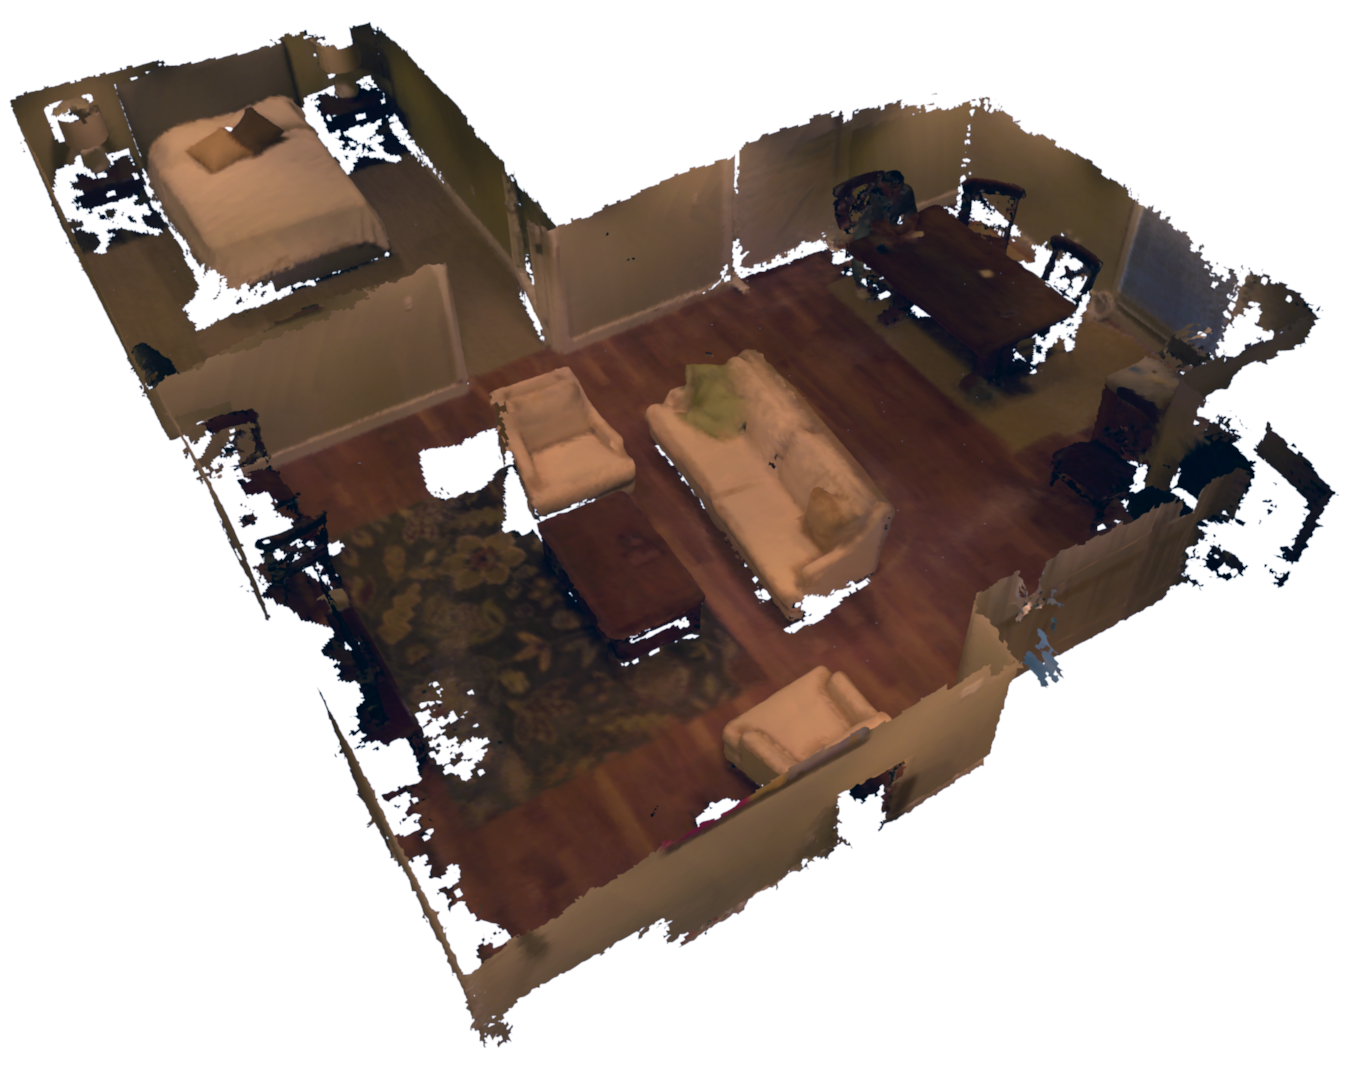
\includegraphics[width=1\textwidth]{img/apartment_scene_color.png}
% 		 \caption{}
% 		 \label{fig:apartment_color} 
% 	 \end{subfigure}
% 	 \begin{subfigure} {0.49\columnwidth} \centering
% 		 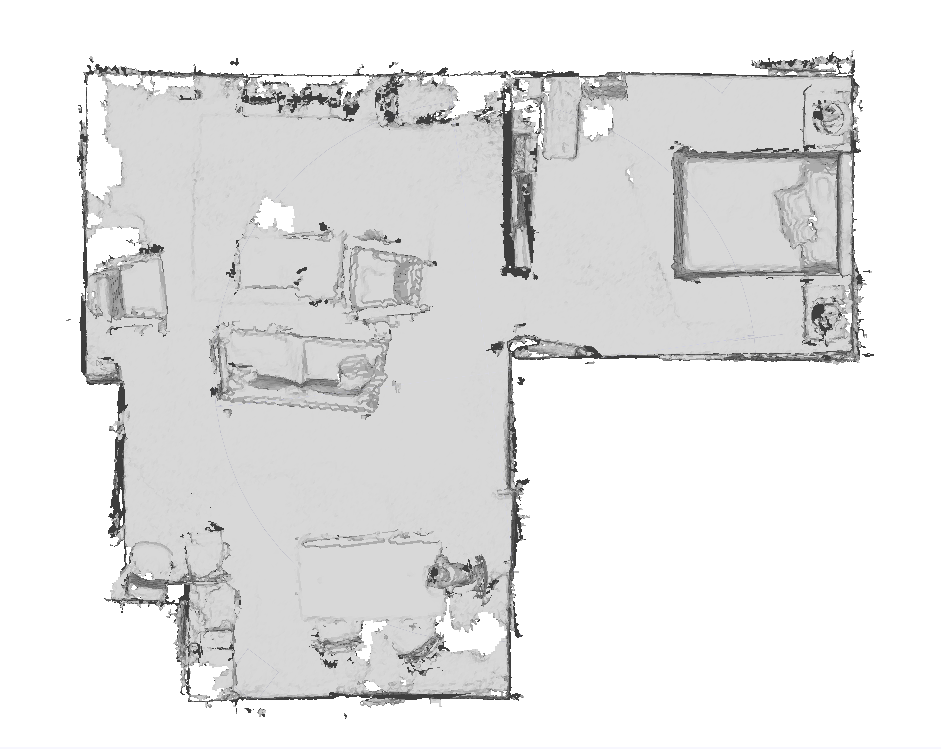
\includegraphics[width=1\textwidth]{img/apartment_scene_topdown_nocolor.png}
% 		 \caption{}
% 		 \label{apartment_scene_topdown_nocolor}
% 	 \end{subfigure}
% 	 \begin{subfigure}{0.49\columnwidth} \centering
% 		 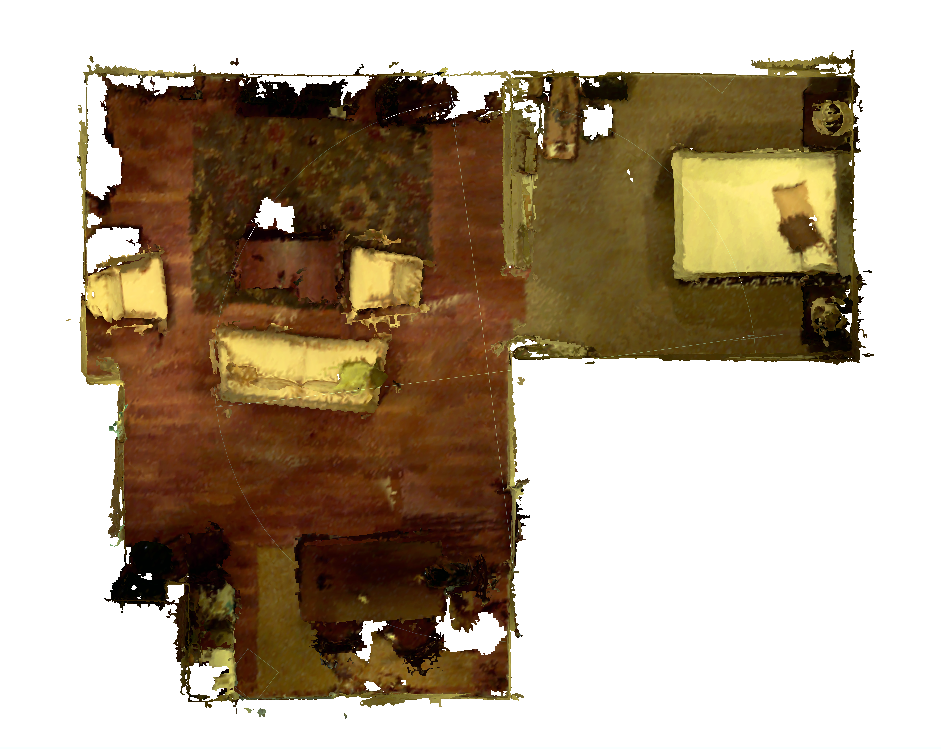
\includegraphics[width=1\textwidth]{img/apartment_scene_topdown_color.png}
% 		 \caption{}
% 		 \label{fig:apartment_scene_topdown_color}
% 	 \end{subfigure}
% % 	 \begin{subfigure} {0.49\columnwidth} \centering
% % 		 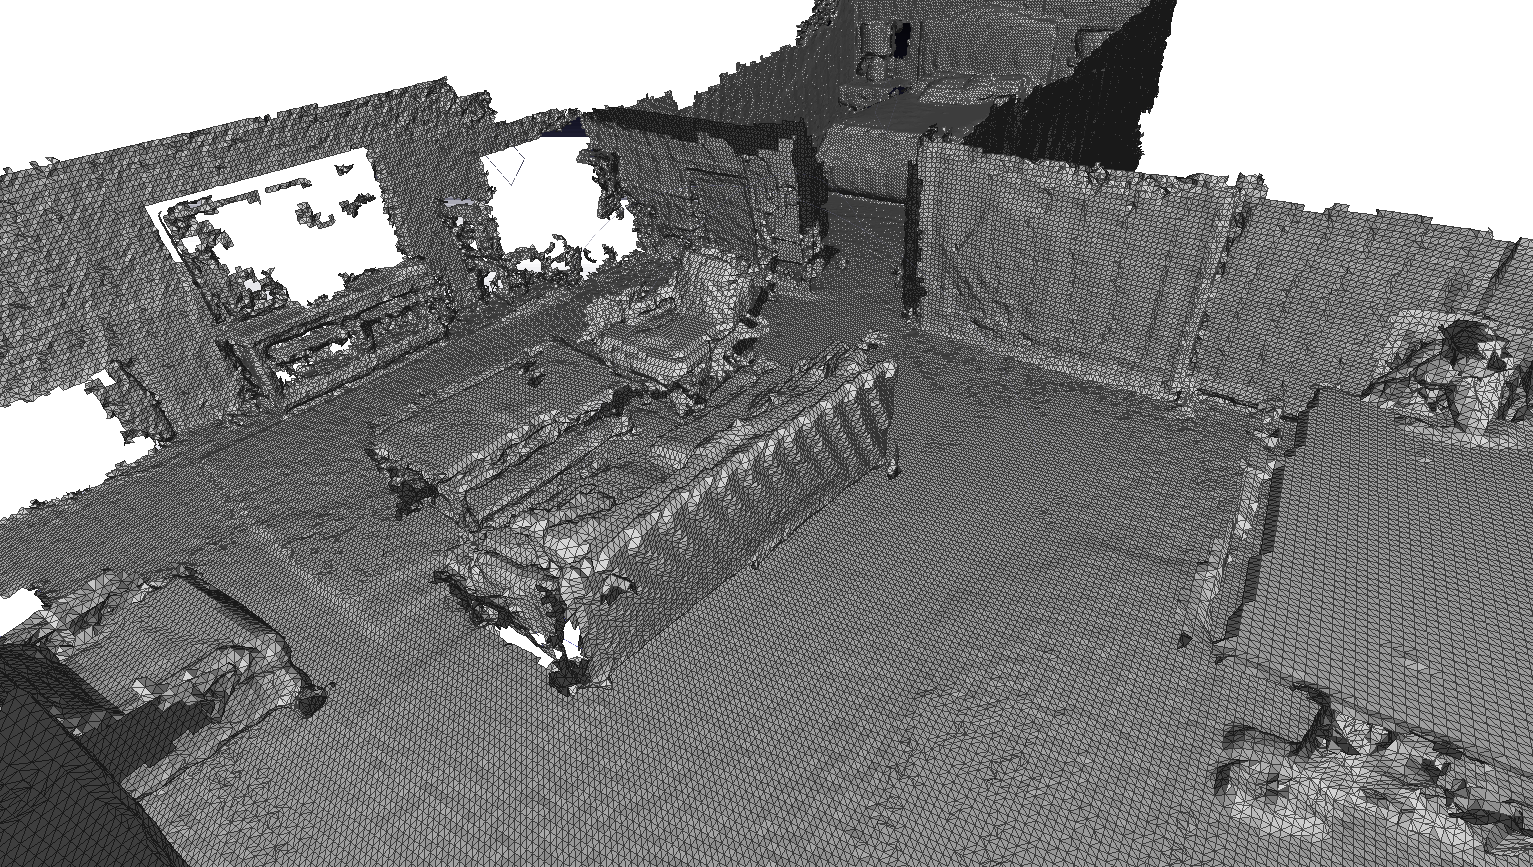
\includegraphics[width=1\textwidth]{img/apartment_scene_closeup_nocolor.png}  
% % 		 \caption{}
% % 		 \label{apartment_scene_closeup_nocolor}
% % 	 \end{subfigure}
% % 	 \begin{subfigure}{0.49\columnwidth} \centering
% % 		 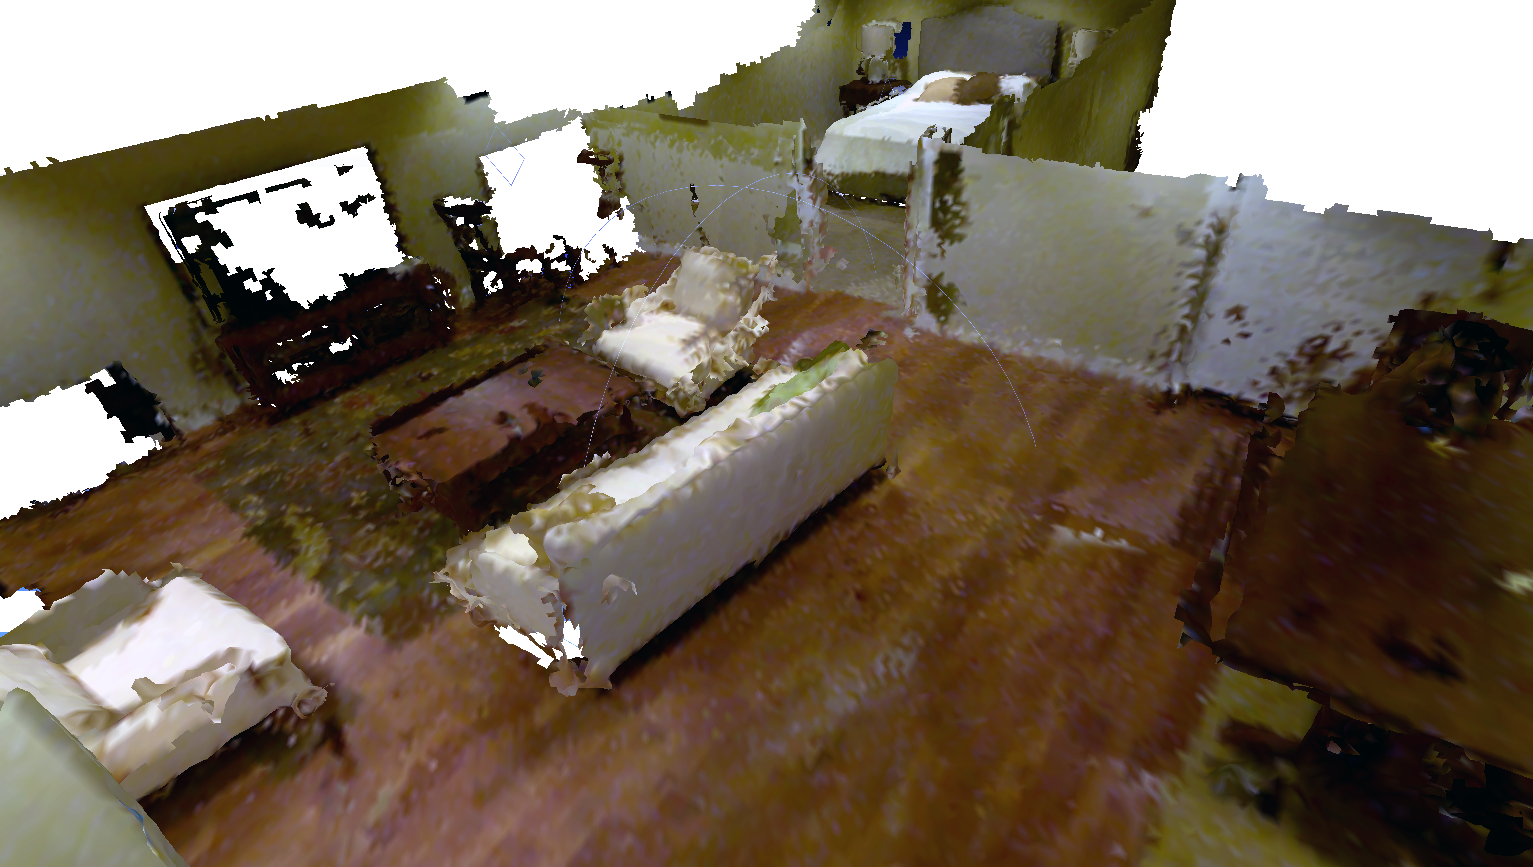
\includegraphics[width=1\textwidth]{img/apartment_scene_closeup_color.png}
% % 		 \caption{}
% % 		 \label{fig:apartment_scene_closeup_color}
% % 	 \end{subfigure}
% 	 \caption{Several views of an apartment scene are shown without and with
% 	 color. These meshes were produced using the tablet device using space
% 	 carving, raycasting, and an offline bundle adjustment procedure to correct
% 	 for pose drift.}
% 	 \label{fig:apartment}
%  \end{figure*}  

%\begin{itemize}
%    \item If we're keeping around the volumetric information, what does that
    % buy us? Can it help us with loop closure?
%    \item These techniques can be used outside of the mobile context to speed
%    things up.
%    \item We gain a lot by using decoupled pose, but there needs to be a way to
 %   incorporate the VIO pose with dense alignment (like they do in Kintinuous).
%\end{itemize}
 
\section{Discussion and Future Work}
Our system is able to create and render large-scale 3D reconstructions of
scenes in real-time using only the limited computational resources of a
\Tango device. We accomplish this without any GPU computing, and use
only the fixed function pipeline to render the scene. We do this out of
necessity to meet the computing requirements of a mobile device. 

Admittedly, our reconstructions are much lower resolution than state-of-the-art
\TSDF mapping techniques, which typically push for sub-centimeter resolution. In
particular, Niessner \etal \cite{NiessnerHashing} produce $4mm$ resolution maps
of comparable or larger size than our own through the use of commodity GPU
hardware and a dynamic spatial hash map. Ultimately, as more powerful mobile
GPUs become available, reconstructions at these resolutions will become
feasible on mobile devices. 

Many previous works \cite{StuecklerSparseDense, niessner2014combining} have
combined sparse keypoint mapping, visual odometry and dense reconstruction to
reduce pose drift. Future research must adapt SLAM techniques combining visual
intertial odometry, sparse landmark localization and dense 3D reconstruction in
a way that is efficient enough to allow real-time relocalization on a mobile device.

% A further area of potential research is in global loop closure and
% relocalization. Whelan \etal\cite{WhelanLoopClose} introduced a means of warping
% the mesh output by \textit{Kintinuous} consistently with global pose updates
%  involving loop closures. But the 3D volumetric data from the \TSDF is lost in
%  this process. Is it possible to warp the \TSDF data directly?

Finally, our task of using onboard \TSDF mapping for aerial robot navigation
remains incomplete. Further work is needed to allow an aerial robot to navigate
autonomously using our system.

% Finally, there is the question of applications. What can be done with a
% real-time dense 3D reconstruction on a mobile device? Applications ranging from
% robot localization and planning to house-scale modelling and augmented reality
% gaming are all possible.

\iffinalcopy
	\section*{Acknowledgements}
	This work was done as part of Google's Advanced Technologies and Projects
	division (ATAP) for \Tango. Thanks to Johnny Lee, Joel Hesch, Esha
	Nerurkar, and Simon Lynen and other ATAP members for their close collaboration
	and support on this project. Thanks to Ryan Hickman for collecting outdoor data.
\fi


\bibliographystyle{IEEEtran}
% argument is your BibTeX string definitions and bibliography database(s)
\bibliography{densemapping, ./densemapping} 
\end{document}
